%
%	Configure LaTeX to produce a PDF "book" using the memoir class
%

\documentclass[10pt,oneside]{memoir}

%
%	Generic Configuration for memoir-based documents
%

\usepackage{layouts}[2001/04/29]


% In case we need a glossary, or index
\usepackage{glossaries}
\glstoctrue
\makeglossaries
\makeindex


% Basic page layout configuration
\def\mychapterstyle{default}
\def\mypagestyle{headings}


% Use 8.5 x 11 inch page layout
\input{../latex/mmd-icanscript-user-guide-layout-8.5x11}


% Use default packages for memoir setup
\input{../latex/mmd-icanscript-user-guide-packages}


% Configure default metadata to avoid errors
\input{../latex/mmd-default-metadata}




\def\mytitle{iCanScript User Guide}
\def\myauthor{Michel Launier}
\def\version{v1.1.2}
\def\email{support@icanscript.com}
%
%	Get ready for the actual document
%

\usepackage[
	colorlinks=true,
    linkcolor=blue!50!green,
    urlcolor=blue,
    citecolor=gray,
	plainpages=false,
	pdfpagelabels,
	pdftitle={\mytitle},
	pagebackref,
	pdfauthor={\myauthor},
	pdfkeywords={\keywords}
	]{hyperref}
\usepackage{memhfixc}


%
%	Configure information from metadata for use in title
%

\ifx\latexauthor\undefined
\else
	\def\myauthor{\latexauthor}
\fi

\ifx\subtitle\undefined
\else
	\addtodef{\mytitle}{}{ \\ \subtitle}
\fi

\ifx\affiliation\undefined
\else
	\addtodef{\myauthor}{}{ \\ \affiliation}
\fi

\ifx\address\undefined
\else
	\addtodef{\myauthor}{}{ \\ \address}
\fi

\ifx\phone\undefined
\else
	\addtodef{\myauthor}{}{ \\ \phone}
\fi

\ifx\email\undefined
\else
	\addtodef{\myauthor}{}{ \\ \email}
\fi

\ifx\event\undefined
\else
	\date[\mydate]{\today}
\fi
\title{\mytitle}
\author{\myauthor}

\ifx\mydate\undefined
\else
	\date{\mydate}
\fi


\ifx\theme\undefined
\else
	\usetheme{\theme}
\fi

\begin{document}

\VerbatimFootnotes


\chapterstyle{\mychapterstyle}
\pagestyle{\mypagestyle}

\newenvironment{tipbox}%
    {%
        \par%
        \centering%
        \color{black!25!gray}%
        \list{}{\leftmargin=0.05\textwidth}%
        \item[]%
        \begin{Sbox}%
        \begin{minipage}{0.93\textwidth}%
    }%
    {\end{minipage}\end{Sbox}\shadowbox{\TheSbox}\endlist}



% Frontmatter
\frontmatter

% Title Page
%\maketitle

\textbf{\Huge User Guide}

\begin{raggedleft}
    \rule{2.5in}{0.4pt}
\end{raggedleft}


\includegraphics[keepaspectratio,width=\textwidth,height=0.75\textheight]{iCanScript_Title.png}

\begin{figure}[htbp]
\centering

\includegraphics[width=256pt,height=256pt]{iCanScriptLogo_256x256x32.png}

\includegraphics[width=256pt,height=38pt]{VisualScriptingForUnity_black.png}
\end{figure}

 
%\clearpage

%
% Copyright Page
%

\vspace*{\fill}
\setlength{\parindent}{0pt}

\ifx\mycopyright\undefined
\else
	\textcopyright{} \mycopyright
\fi

\begin{center}
	\framebox{ \parbox[t]{1.5in}{\centering Formatted for \LaTeX \\ 
	by MultiMarkdown}}
\end{center}

\setlength{\parindent}{1em}
\clearpage

\tableofcontents
%\listoffigures
%\listoftables


\mainmatter

\setlength{\parskip}{1em}




\pagebreak 

\part{Introduction}
\label{introduction}

\chapter{What is iCanScript?}
\label{whatisicanscript}

\begin{quote}

\leftskip=0.5\textwidth

Think twice before you start programming or you will program twice before you start thinking. 

\noindent\makebox[0.5\linewidth]{\rule{0.5\linewidth}{0.4pt}}

- Unknown
\end{quote}



More then 50 years after ENIAC\footnote{ENIAC (Electronic Numerical Integrator And Computer) was the first electronic general-purpose computer. It was Turing-complete, digital, and capable of being reprogrammed to solve a full range of computing problems.}, most programmers still rely solely on textual editors to express their creative thoughts into programs that can be compiled or interpreted by computers.

As the programs increase in complexity, many corporations encourage the interdisciplinary\footnote{The term interdisciplinary is used to express a team composed of various expertise or talent not limited to software engineering.} discussion of the high-level concepts overseeing the software product to be created. In all cases, these high-level concepts are expressed in diagrams for it is the simplest and most direct way of building and iterating on those fundamental aspects of the product. It is this trend to graphically convey software concepts that conducted to the creation of iCanScript.

iCanScript is part of a new breed of visual editors that focuses on expressing programmatic behaviour using nodal diagrams. It integrates with existing toolsets extending the text editor for writing Unity\footnote{Unity is a trademark of Unity Technologies.} scripts. It offers a visual workflow to build, review, and publish programming logic preserving the ability to write low-level logic using your favourite coding software.

\chapter{Feature Overview}
\label{featureoverview}

\begin{itemize}
\item Fully integrated functional \& state chart diagrams;

\item Unlimited nesting of nodes allows for structured visual scripts;

\item Visual scripts can be saved and loaded to\slash from Prefabs to create your own personal visual library;

\item Each node can be displayed as:

\begin{itemize}
\item unfolded (displays nested nodes);

\item folded (hides nested nodes) or;

\item iconized.

\end{itemize}

\item Visual Editor zoom in\slash out enables bird's-eye view and eases navigation of large diagrams;

\item Visual library includes Unity's runtime functionality;

\item Library can be expanded with your own scripts and external packages;

\item Auto-save when scene is saved;

\item Auto-compiled when application is started;

\item Port values are displayed in real-time when the application is executing;

\item Available for Standard and Professional versions of Unity.

\end{itemize}

\chapter{When to use Visual Scripts?}
\label{whentousevisualscripts}

Our goal in creating iCanScript is to simplify and accelerate scripting within Unity's development environment. iCanScript offers a visual alternative to traditional textual scripts enabling greater accessibility for both programmers and non-programmers.

We believe that depicting the scripts allows for a larger community of talents to interact with the high-level logic that drive your games. It simplifies the understanding of the overall structure to all individuals in your production.

\emph{So can visual scripts replace all textual scripts in a production?}

Probably not{\ldots} The fact is that visual and textual scripts have different strengths and weaknesses.

Visual scripts excel at summarizing complex interactions that typically span multiple source files when implemented using textual scripts. These interactions include:

\begin{itemize}
\item mission control logic;

\item behaviour state charts;

\item gameplay logic; and

\item any high-level functional diagrams.

\end{itemize}

Textual scripts are best at expressing tight calculations that can be implemented in a single source file. The textual scripts can thereafter be integrated into iCanScript as building blocks of high-level logic. These algorithms include:

\begin{itemize}
\item calculation loops;

\item search loops;

\item complex mathematical expressions; and

\item large selectors (switch-case).

\end{itemize}

We hope that you find the right balance in using iCanScript combined with traditional scripting methods to increase productivity and, more importantly, \emph{HAVE MORE FUN} in writing your scripts.

\chapter{Who will Benefit from Using iCanScript?}
\label{whowillbenefitfromusingicanscript}

\underline{\textbf{The Novice and Intermediate Programmer:}} The novice programmer will greatly benefit from the immense Unity library available for visual scripting. The programmer will find enjoyable the ability to create \emph{\textbf{state charts}} and \emph{\textbf{data flow diagrams}} in a visual and coherent environment. The ability to \emph{\textbf{aggregate multiple functions and state charts}} into a \emph{\textbf{package node}} combined with the \emph{\textbf{unlimited nesting}} capabilities of iCanScript provides a sandbox to design at multiple levels of abstraction.

\underline{\textbf{The Expert Programmer:}} For the expert programmer, iCanScript \emph{\textbf{complements textual scripting with visual scripting}}. Using .NET reflection and optional meta-attributes, textual scripts can easily be published to the iCanScript library. Therefore, the \emph{\textbf{programmer remains in full control over the scripting workflow}} deciding when and where visual scripting benefits the overall project.

\underline{\textbf{Non-Technical Individual:}} iCanScript visual environment greatly simplifies the \emph{\textbf{understanding of script structure}} for all individuals including non-technical individuals. By removing the ``needy greedy'' details of programming languages, iCanScript allows the \emph{\textbf{non-technical individual to create or modify simple scripts}}. The creation of large and maintainable scripts require a minimal knowledge of programming structures (even with visual scripting) and may prove to be challenging for non-technical individuals.

\pagebreak 

\part{Installation \& Upgrade}
\label{installationupgrade}

\chapter{Installation}
\label{installation}
\begin{tipbox}
\color{red}

Please note that the installation of iCanScript from the Unity Asset Store is currently not discussed. It will be added in future releases of this document.

\end{tipbox}




\includegraphics[width=32pt,height=32pt]{Drive-Download_48x48.png} iCanScript is a downloadable plugin for the Unity 3D game engine. It comes in the form of a Unity package that must be installed for each project.

The initial download of iCanScript is available from the project \href{http://www.icanscript.com}{website}\footnote{\href{http://www.icanscript.com}{http:/\slash www.icanscript.com}}. User registration is required to obtain the latest version of the iCanScript software via email. An overview of the registration, download and installation procedure is available in the following video:

\href{http://youtu.be/LJIqMaUNoAU}{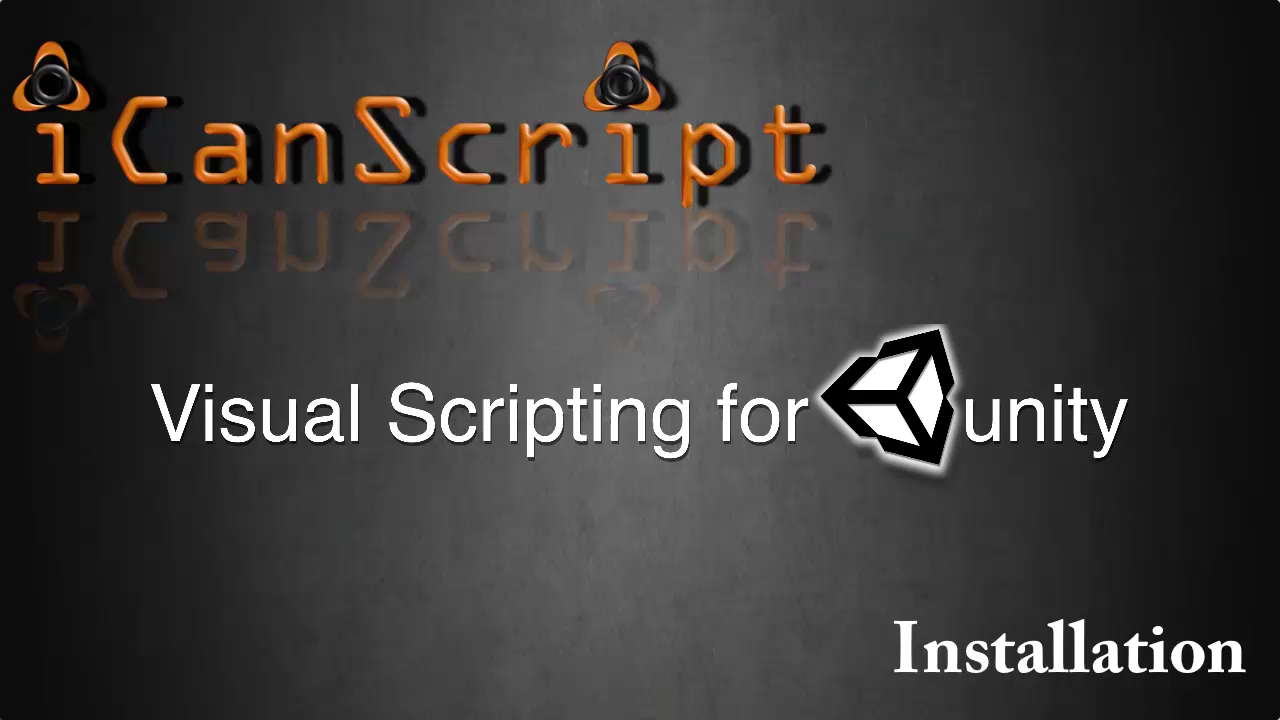
\includegraphics[width=320pt,height=180pt]{tutorial-installation-tumbnail.png}}\footnote{\href{http://youtu.be/LJIqMaUNoAU}{http:/\slash youtu.be\slash LJIqMaUNoAU}}

Follow these steps to install iCanScript for the first time:

\begin{enumerate}
\item Visit the iCanScript web site at \href{http://www.icanscript.com}{www.icanscript.com};

\item Click the download button from the home page;

\item Fill-in the registration form (the email is important);

\item Shortly after, you will receive an email with the latest version of iCanScript in attachment;

\item Open the email and save the iCanScript package;

\item Launch Unity and import the iCanScript package (see Figure \ref{custom-import.png});

\item You are now ready to start …

\end{enumerate}

\begin{figure}[htbp]
\centering
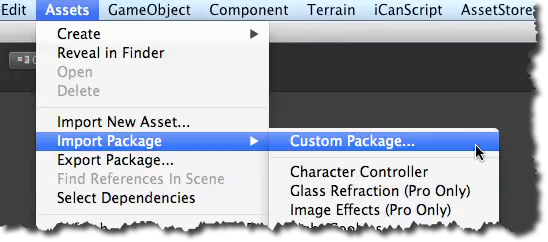
\includegraphics[keepaspectratio,width=\textwidth,height=0.75\textheight]{custom-import.png}
\caption{Importing iCanScript into Unity.}
\label{custom-import.png}
\end{figure}

You now have the knowledge to download and install iCanScript in your own project. I propose that you move on to the [quick start tutorial][] where you will build your first visual script.
\begin{tipbox}


\includegraphics[width=32pt,height=32pt]{icanscript-ui-tips_64x64x32.png} {\Large \color{black} iCanScript User Interface Tips }

\begin{center}\rule{\textwidth}{0.4pt}\end{center}

\begin{quote}

Subsequent software releases can be downloaded using the upgrade (\autoref{upgradingicanscript}) feature of iCanScript.
\end{quote}

\end{tipbox}



\chapter{Removing iCanScript}
\label{removingicanscript}

The following steps are needed to uninstall iCanScript from your project:

\begin{itemize}
\item Remove the \emph{\textbf{iCanScript}} folder;

\item Open the \emph{Gizmos} folder and remove the \emph{\textbf{iCanScriptGizmo.png}} file;

\item Remove the optional \emph{\textbf{iCanScript\_Nodes}} package;

\end{itemize}
\begin{tipbox}


\includegraphics[width=32pt,height=32pt]{PostitNote_48x48.png} \textbf{Note:} Uninstalling the previous version of iCanScript is required when performing an upgrade.

\end{tipbox}



\begin{figure}[htbp]
\centering
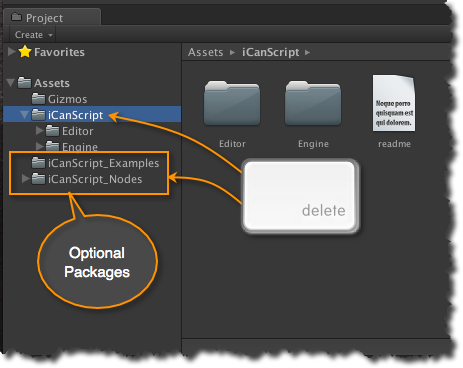
\includegraphics[keepaspectratio,width=\textwidth,height=0.75\textheight]{remove-packages.png}
\caption{Uninstalling the iCanScript packages.}
\label{remove-packages.png}
\end{figure}

\begin{figure}[htbp]
\centering
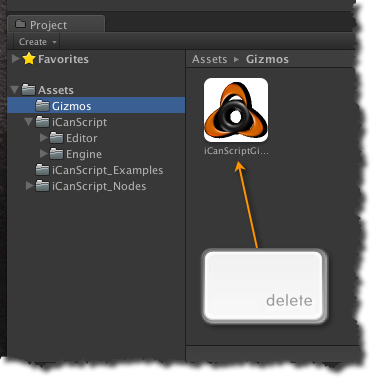
\includegraphics[keepaspectratio,width=\textwidth,height=0.75\textheight]{remove-gizmo.png}
\caption{Removing the iCanScript Gizmo.}
\label{remove-gizmo.png}
\end{figure}

\chapter{Upgrading iCanScript}
\label{upgradingicanscript}

Improvements to iCanScript are regularly made available as downloadable software updates. 

The following steps are needed to verify for and update to the latest version of iCanScript:

\begin{enumerate}
\item Verify for an update using the menu item: \begin{color}{blue!70!red}\emph{\textbf{Help->iCanScript->Check for Updates…}}\end{color};

\item If an update is available, a dialog box will guide you to the download page;

\item Download the latest version of iCanScript;

\item Open Unity and uninstall the current version of iCanScript (see Removing iCanScript (\autoref{removingicanscript}));

\item Import the latest version of iCanScript (see Installation (\autoref{installation}));

\item An alert box will be shown if data conversion is required after the upgrade;

\begin{itemize}
\item data conversion is performed in memory;

\item each visual script data is converted independently;

\item converted data is persisted when the scene is saved;

\item data rollback is performed if scene is not saved after an upgrade.

\end{itemize}

\item Save the scene to complete the upgrade.

\end{enumerate}

\begin{figure}[htbp]
\centering
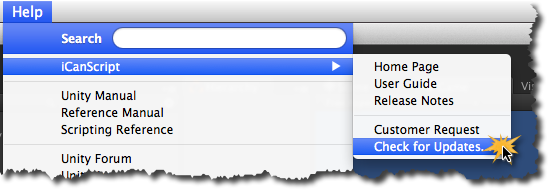
\includegraphics[keepaspectratio,width=\textwidth,height=0.75\textheight]{ics-check-for-update.png}
\caption{Verifying for an update.}
\label{ics-check-for-update.png}
\end{figure}

\pagebreak 

\part{Visual Script Anatomy}
\label{visualscriptanatomy}

\chapter{Nodes, Ports, and Bindings}
\label{nodesportsandbindings}

A good understanding of the fundamental building blocks of a visual script is necessary to effectively use iCanScript.

A visual script includes three (3) types of component being:

\begin{itemize}
\item \textbf{Nodes};

\item \textbf{Ports}; and {\ldots}

\item \textbf{Bindings.}

\end{itemize}

\begin{figure}[htbp]
\centering
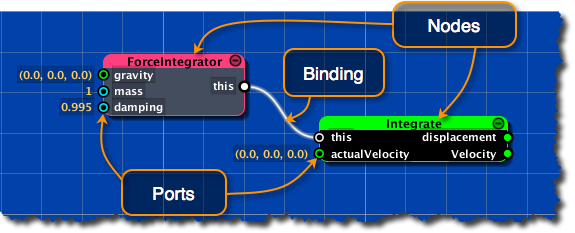
\includegraphics[keepaspectratio,width=\textwidth,height=0.75\textheight]{ics-visual-script-building-blocks.png}
\caption{Visual Script Building Blocks.}
\label{ics-visual-script-building-blocks.png}
\end{figure}

The \textbf{node} is the primary ingredient of visual scripts. Its main purpose is to encapsulate various type of behaviours such as:

\begin{itemize}
\item variables \& functions;

\item algorithms;

\item states and state charts; and

\item nested visual scripts (i.e. packages or submodules).

\end{itemize}

The \textbf{ports} are the public interfaces to nodes. Multiple ports may exist on the same node each representing a distinct interface. A single port is directional and is either an input port or an output port both never both. The ports are further classified as:

\begin{itemize}
\item \emph{data flow:} feeding or extracting data to\slash from the node behaviour;

\item \emph{control flow:} controlling the execution state of the node (\emph{boolean} value);

\item \emph{state transition:} controlling the state transition triggers (state charts only).

\end{itemize}

The \textbf{bindings} define relationships between ports. Bindings can only be created between compatible ports. Furthermore, bindings are directional and can only exist between an output port and one or more inputs port(s). That is, connecting input ports together or output ports together is not permitted. The following summarizes the permissible bindings:

\begin{itemize}
\item from an output data port to one or more input data or control port(s) if the data type is compatible;

\item from an output control port to one or more input data or control port(s) if the data type is compatible with a \emph{boolean} value;

\item from an output state port to one input state port using a transition trigger module.

\end{itemize}

\underline{\textbf{Exception:}} iCanScript includes a special port, named the \emph{Multiplexer Port}, that bridges multiple output ports into a single output port. This port is especially useful when multiple exclusive execution paths of a visual script must combine into a single set of data values. (see Data Flow Diagram (\autoref{dataflowdiagram}) for additional details).
\begin{tipbox}


\includegraphics[width=33pt,height=33pt]{iCanScriptLogo_32x32x32.png} {\Large \color{black} iCanScript Advanced Topic }

\begin{center}\rule{\textwidth}{0.4pt}\end{center}

iCanScript internally implements the \emph{Multiplexer Port} using a specialized \emph{data multiplexer node}. For convenience to the user, this multiplexer node is always iconized and positioned on the edge of the parent node giving the illusion of being a \emph{multiplexer port}.

\end{tipbox}



\chapter{Node Anatomy}
\label{nodeanatomy}

The \emph{node} is by far the most elaborate component of visual scripts. It plays a key role in the structure, execution, and layout of the visual script.

All nodes in iCanScript share a common set of attributes:

\begin{itemize}
\item \textbf{Name:} A character string representation of the node;

\item \textbf{Type:} Identifies the node specialization.

\item \textbf{Tree-like Hierarchical Structure:}

\begin{itemize}
\item A parent node;

\item Zero or more child components:

\begin{itemize}
\item \emph{Ports};

\item \emph{Child Nodes} (nested Visual Script).

\end{itemize}

\end{itemize}

\item \textbf{Graphical Representation:} (see figure \ref{ics-hierarchy-tree-example.png}

\begin{itemize}
\item Position within the parent node;

\item Display State:

\begin{itemize}
\item \emph{Unfolded};

\item \emph{Folded}; or

\item \emph{Iconized}.

\end{itemize}

\end{itemize}

\end{itemize}

The following image depicts an unfolded node as seen in the \emph{Visual Editor}:

\begin{figure}[htbp]
\centering
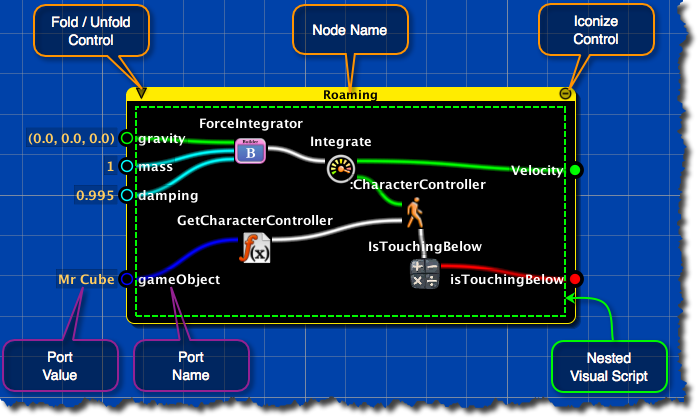
\includegraphics[keepaspectratio,width=\textwidth,height=0.75\textheight]{ics-anatomy-of-a-node.png}
\caption{Anatomy of an unfolded node as seen in the \emph{Visual Editor}.}
\label{ics-anatomy-of-a-node.png}
\end{figure}

The following image depicts the same unfolded node as seen in the \emph{Tree View}:

\begin{figure}[htbp]
\centering
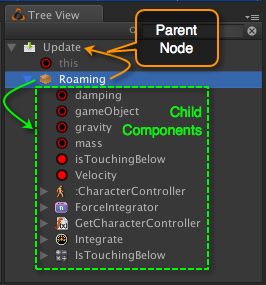
\includegraphics[keepaspectratio,width=\textwidth,height=0.75\textheight]{ics-hierarchy-tree-example.png}
\caption{Anatomy of an unfolded node as seen in the \emph{Tree View}.}
\label{ics-hierarchy-tree-example.png}
\end{figure}

\begin{enumerate}
\item \textbf{Node Name:} User configurable name for the node. The name is editable in the inspector or the hierarchy tree. The programmatic function \slash  type name is used by default.

\item \textbf{Iconize Control:} Clicking this pictogram causes the node to take its iconic representation.

\item \textbf{Fold\slash Unfold Control:} Clicking this pictogram toggles the node between its folded and unfolded representation. The fold\slash unfold control is available only for those node types that can contain nested visual scripts. (see [Node Types] for details).

\item \textbf{Node Ports:} Ports are positioned on any of the four node edges.

\begin{itemize}
\item \emph{Port Name} is displayed inside the node;

\item \emph{Port Value} is display outside the node.

\end{itemize}

\item \textbf{Nested Visual Script:} The central area of the node is used to manage the nested child nodes. The child node container is only visible when the node is unfolded. See section [Node Types] for details on which node types support nested children.

\end{enumerate}

\chapter{Specialized Nodes}
\label{specializednodes}

The nodes come in various types or specialization. For example, their is a specialization that represents \emph{Variables}, another that represents \emph{Functions} and yet another for \emph{Message Handlers}. 

\chapter{Port Types}
\label{porttypes}

\chapter{Node Nesting}
\label{nodenesting}

\chapter{Data Flow Diagram}
\label{dataflowdiagram}

\chapter{State Chart Diagram}
\label{statechartdiagram}

\section{States}
\label{states}

\subsection{Entry Function}
\label{entryfunction}

\subsection{Update Function}
\label{updatefunction}

\subsection{Exit Function}
\label{exitfunction}

\subsection{Nested State}
\label{nestedstate}

\section{Transitions}
\label{transitions}

\subsection{Trigger Function}
\label{triggerfunction}

\subsection{Transition Behaviour}
\label{transitionbehaviour}

\pagebreak 

\part{Integration with Unity}
\label{integrationwithunity}

\chapter{Unity Integration}
\label{unityintegration}

iCanScript is designed to seamlessly integrated into the Unity development environment. It builds on the philosophies and application programming interfaces (APIs) available to Unity script programmers.

iCanScripts integrates with the following Unity concepts:

\begin{itemize}
\item Visual scripts are standard Unity \emph{Components};

\item Each visual script is compiled into an Unity \emph{Behaviour} and executed as such;

\item All Unity engine programming interfaces are available in the iCanScript library database;

\item All \emph{Behaviour Messages} are implemented as \emph{Message Handler Nodes};

\item Visual script libraries are implemented with Unity \emph{Prefabs};

\item Visual scripts are saved and loaded with the game object they are attached to;

\item Visual scripts are compiled when starting the Unity engine.

\end{itemize}

iCanScript extends the Unity Concepts with:

\begin{itemize}
\item Functional diagrams;

\item State Chart diagrams;

\item Automatic data driven execution sequencing;

\item Automatic deadlock avoidance.

\end{itemize}
\begin{tipbox}

 
\includegraphics[width=33pt,height=33pt]{PostitNote_32x32.png} \textbf{Note:} Proper usage of iCanScript requires minimal knowledge of the Unity platform.

\end{tipbox}



\chapter{Adding a Visual Script}
\label{addingavisualscript}

To use iCanScript, you first need to install a visual scripts on one of your game objects. To illustrate this process, we will add a visual script to a sphere that will later be used as a trigger zone. 

To do so, you must:

\begin{enumerate}
\item Select a game object to contain the visual script;

\item Create a visual script using the menu item: \begin{color}{blue!70!red}\emph{\textbf{iCanScript->Create Visual Script}}\end{color}.

\end{enumerate}

\begin{figure}[htbp]
\centering
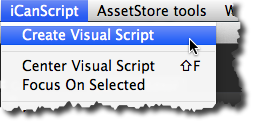
\includegraphics[keepaspectratio,width=\textwidth,height=0.75\textheight]{ics-menu-create-visual-script.png}
\caption{Create Visual Script menu item.}
\label{ics-menu-create-visual-script.png}
\end{figure}

\emph{Et voilà, you have a visual script !!!} It does not do anything yet but it is ready to listen and react to Unity messages. We will look at defining and handling Unity messages in the next section. For now, let's examine the changes brought when creating the visual script.

When iCanScript creates a visual script, it attaches two (2) Unity script components on the game object. These components are:

\begin{enumerate}
\item \emph{\textbf{iCS\_VisualScript (persistent storage)}}

\item \emph{\textbf{iCS\_Behaviour (runtime compiler \& execution services)}}

\end{enumerate}

\begin{figure}[htbp]
\centering
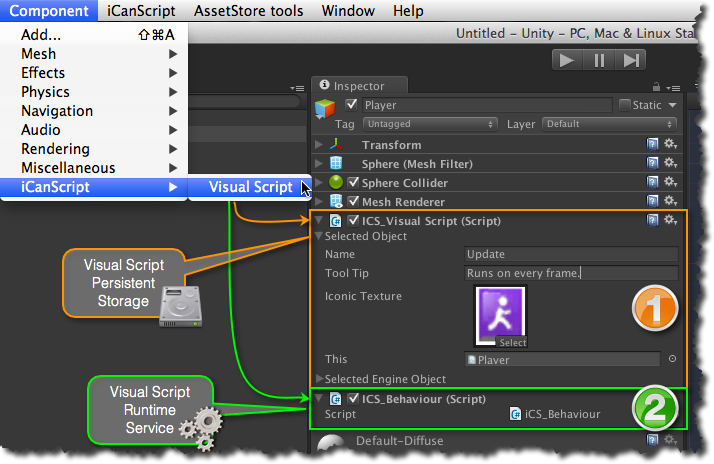
\includegraphics[keepaspectratio,width=\textwidth,height=0.75\textheight]{icanscript-components.png}
\caption{iCanScript visual script components.}
\label{icanscript-components.png}
\end{figure}


\includegraphics[width=32pt,height=30pt]{stamp-1-orange.png} The \emph{iCS\_VisualScript} contains the visual script persistant data including the definitions of nodes, ports, bindings as well as their layout information. It is populated and modified by the iCanScript editors.


\includegraphics[width=32pt,height=30pt]{stamp-2-green.png} The \emph{iCS\_Behaviour} is dynamically created from the visual script data and includes the source code for the message handlers of the visual script. It uses the execution services of the iCanScript engine library (i.e. iCanScriptEngine.dll) to manage the execution flow and resolve data contention (also known as deadlocks).
\begin{tipbox}

\textbf{Note:} You must delete the \emph{iCS\_VisualScript} component to remove the visual script from the game object. The \emph{iCS\_Behaviour} component will be re-created if you delete it while the \emph{iCS\_VisualScript} is installed.

\end{tipbox}



\chapter{Libraries \& Prefabs}
\label{librariesprefabs}

Visual script libraries are created using Unity’s Prefab concept. 

\pagebreak 

\part{How To}
\label{howto}

\part{Example Project}
\label{exampleproject}

\chapter{Objective}
\label{objective}

In this section, we examine the core constructs of iCanScript with the help of a small example. To that end, we shall first establish the working parameters of our example by creating a storyline and setting up the scene before implementing the visual scripts.

The following is a summary of the steps to build our first example:

\begin{enumerate}
\item Create a storyline (\autoref{storyline}) to define the working parameters for our example;

\item Identify and define the actors (\autoref{ouractors}) for our story;

\item Build a scene in Unity populated with the defined actors (\autoref{ouractors});

\item Design the visual script for moving Mr Cube (\autoref{movingmrcubestep1});

\item Design the visual script for enabling \& disabling Ms Light (\autoref{enablingdisablingmslight});

\item Complete the example by adding a Panic State (\autoref{addingapanicstate}) for Mr Cube.

\end{enumerate}

\chapter{Storyline}
\label{storyline}

If you are like me, you prefer learning the workings of a tool in the context of a small example. Like all good game designers, I like to give a soul to my project using a storyline. We can then extract working scenarios to direct the creation of our visual scripts.

Here goes the story:

\begin{quote}

In the land of Emptiness lives Mr Cube. Mr Cube has a busy life roaming around on an invisible 2D plane. Since Mr Cube is a close relative of Mr Fly, he is attracted to Ms Light that also lives in the land of Emptiness. Little does Mr Cube know is that Ms Light is shy and she get ``turned off'' if anyone comes to close to her. When in the dark, Mr Cube panics and runs around in all directions. Luckily for Mr Cube, Ms Light gets ``turned on'' when Mr Cube is far enough from her.
\end{quote}

(Wow! we got romance, terror and deception. What a great plot!)

\chapter{Our Actors}
\label{ouractors}

Before creating visual scripts, we first need to build a scene in Unity and populate it with actors. Based on the storyline, the actors are (the camera has been purposely omitted):

\begin{itemize}
\item \textbf{Mr. Cube} (I'll let you guess the shape to use);

\item \textbf{Ms. Light} (a directional light);

\item \textbf{Near Trigger Zone} to turn off \emph{Ms. Light} (a sphere will do fine);

\item \textbf{Far Trigger Zone} to turn on \emph{Ms. Light} (again a sphere will do fine).

\end{itemize}

The main characteristics of the actors are:

\begin{itemize}
\item All actors live on a 2D plane with the Y-axes set to zero (0);

\item Ms. Light and both Trigger Zones are centred at (0,0,0);

\item Both Trigger Zones are configured to trigger when colliding with \emph{Rigid Bodies};

\item The Near Trigger Zone will be 2 meters in diameter;

\item The Far Trigger Zone will be 3 meters in diameter;

\item Mr. Cube is one meter in dimensions;

\item Mr. Cube includes a \emph{Rigid Body} component to generate collision triggers.

\end{itemize}

You may ask yourself why two trigger zones? We want to avoid \emph{Ms Light} from rapidly transitioning on and off while \emph{Mr Cube} nears her. If only one trigger zone existed, \emph{Mr Cube} could navigate on the edge of the trigger zone causing \emph{Ms Light} to flicker. By creating a buffer area between the on trigger (near) and the off trigger (far), we remove the possibility of \emph{Ms Light} flickering.

\chapter{Creating the Unity Project}
\label{creatingtheunityproject}

We are now ready to build our scene in Unity. First, we need a fresh new Unity project with an installed version of iCanScript. For the purpose of this tutorial, the project will be named ``Houpi Youpi'' (I don't know how to call it! So please bear with me{\ldots}).

Open Unity and select the \begin{color}{blue!70!red}\emph{\textbf{File->New Project...}}\end{color} menu item as shown in the image below:

\begin{figure}[htbp]
\centering
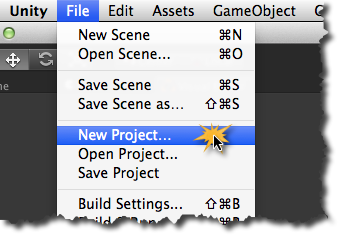
\includegraphics[keepaspectratio,width=\textwidth,height=0.75\textheight]{unity-new-project.png}
\caption{Create a new Unity project.}
\label{unity-new-project.png}
\end{figure}

Next you will be asked for a project name and prompted to install standard Unity packages. Enter \emph{``HoupiYoupi''} as the project name. None of the Unity packages will be required for this tutorial. So don't select any and close the dialog box by clicking the \begin{color}{blue!70!red}\emph{\textbf{Create Project}}\end{color} button.

\begin{figure}[htbp]
\centering
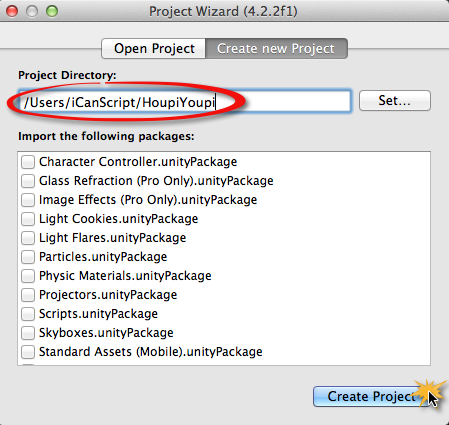
\includegraphics[keepaspectratio,width=\textwidth,height=0.75\textheight]{create-houpi-youpi.png}
\caption{Create \emph{Houpi Youpi} Project.}
\label{create-houpi-youpi.png}
\end{figure}

You now have a bare project in which to import iCanScript. Please follow the instructions in the installation (\autoref{installation}) section to download the latest version of iCanScript if you haven't already done so. Use the \begin{color}{blue!70!red}\emph{\textbf{Assets->Import Package->Custom Package...}}\end{color} menu item to import iCanScript into your project. Once you complete the import, your project panel in Unity should look as follows: 

\begin{figure}[htbp]
\centering
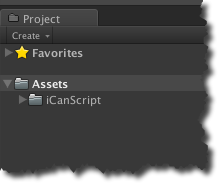
\includegraphics[keepaspectratio,width=\textwidth,height=0.75\textheight]{icanscript-empty-project.png}
\caption{Unity project with the iCanScript package.}
\label{icanscript-empty-project.png}
\end{figure}

\clearpage

\section{Adding Actors to the Scene}
\label{addingactorstothescene}

Ok, we are ready to bring our actors into the scene. For each new project, Unity creates a default scene with the main camera object. You will add the actors to the default scene using the \begin{color}{blue!70!red}\emph{\textbf{GameObject->...}}\end{color} menu.

\subsection{Ms Light}
\label{mslight}

Let's start by adding \emph{Ms Light}. Select the \begin{color}{blue!70!red}\emph{\textbf{GameObject->Create Other->Directional Light}}\end{color} menu item and, \emph{swoosh {\ldots} Ms Light} appears.

\begin{figure}[htbp]
\centering
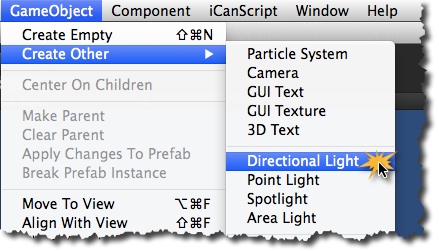
\includegraphics[keepaspectratio,width=\textwidth,height=0.75\textheight]{adding-directional-light.png}
\caption{Adding Ms Light to the scene.}
\label{adding-directional-light.png}
\end{figure}

Double click on the \emph{``Directional light''} label in the hierarchy panel to rename it to \emph{``Ms Light''}. Because \emph{Ms Light} is a directional light, she lights the scene equally regardless of her position. For consistency shake with our story, I suggest you position her at (0,0,0) as show in Figure \ref{config-mrs-light.png}.

\begin{figure}[htbp]
\centering
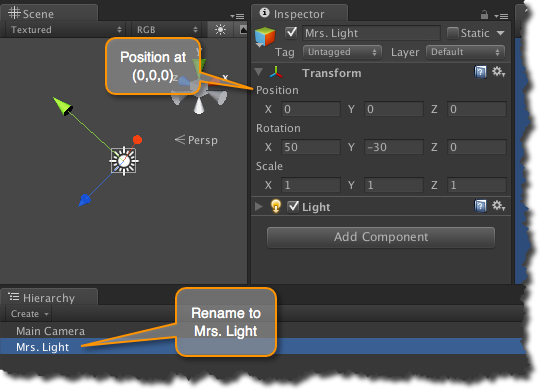
\includegraphics[keepaspectratio,width=\textwidth,height=0.75\textheight]{config-mrs-light.png}
\caption{Renaming and positioning Ms Light.}
\label{config-mrs-light.png}
\end{figure}
\begin{tipbox}


\includegraphics[width=33pt,height=33pt]{UnityLogo_32x32.png} {\Large \color{black} Unity Tips }

\begin{center}\rule{\textwidth}{0.4pt}\end{center}

\textbf{What's a Directional Light?}

\begin{quote}

A \textbf{directional light} illuminates the scene with uniform intensity regardless of the distance from the light source. It is often used to simulate the sun. Its light direction and color can be configured to create various time-of-day effects and neat extra-terrestrial atmospheres. The default color and direction of the directional light source is adequate for our example.
\end{quote}

\end{tipbox}



\subsection{Near \& Far Trigger Zones}
\label{nearfartriggerzones}

The two trigger zones are spheric in shape and are create with the \begin{color}{blue!70!red}\emph{\textbf{GameObject->Create Other->Sphere}}\end{color} menu.

\begin{figure}[htbp]
\centering
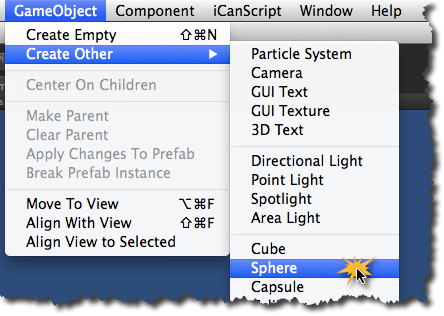
\includegraphics[keepaspectratio,width=\textwidth,height=0.75\textheight]{adding-trigger-zones.png}
\caption{Adding Trigger Zones to the Scene.}
\label{adding-trigger-zones.png}
\end{figure}

After you have created both \emph{trigger zones}, you need to configure them as follows:

\begin{enumerate}
\item Name one of them \emph{``Near Trigger Zone''} and the other \emph{``Far Trigger Zone''};

\item As for \emph{Ms Light}, position both trigger zones at (0,0,0);

\item Now resize the \emph{``Near Trigger Zone''} to 2 meters and the \emph{``Far Trigger Zone''} to 3 meters by setting the scale to (2,2,2) and (3,3,3) respectively;

\item The final step is to enable the \textbf{trigger} behaviour of both spheres. This is realized by clicking the \begin{color}{blue!70!red}\emph{\textbf{Is Trigger}}\end{color} checkbox in the \emph{Sphere Collider} component of the trigger zones (see \ref{config-trigger-zones.png}).

\end{enumerate}

\begin{figure}[htbp]
\centering
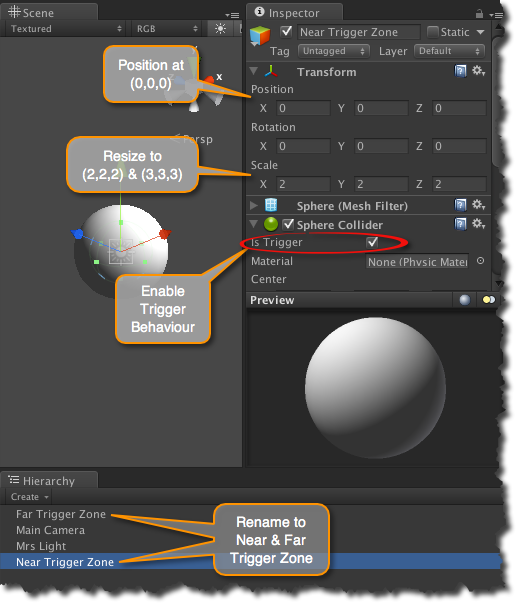
\includegraphics[keepaspectratio,width=\textwidth,height=0.75\textheight]{config-trigger-zones.png}
\caption{Configuring Near \& Far Trigger Zones.}
\label{config-trigger-zones.png}
\end{figure}

\subsection{Mr Cube}
\label{mrcube}

We are now ready for our final actor: \emph{Mr Cube}. Use the \begin{color}{blue!70!red}\emph{\textbf{GameObject->Create Other->Cube}}\end{color} menu item to add \emph{Mr Cube} to the scene.

\begin{figure}[htbp]
\centering
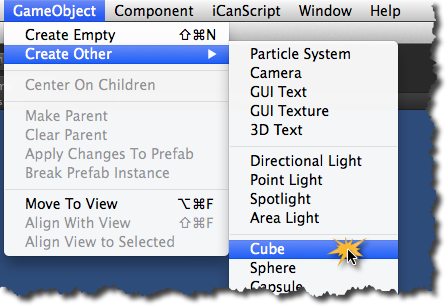
\includegraphics[keepaspectratio,width=\textwidth,height=0.75\textheight]{adding-mr-cube.png}
\caption{Adding Mr Cube to the scene.}
\label{adding-mr-cube.png}
\end{figure}

Once more, you need to set the initial parameters of the new actor. \emph{Mr Cube} must be configured as follows:

\begin{enumerate}
\item Rename the cube object to \emph{``Mr Cube''} (sexy!);

\item Relocate \emph{Mr Cube} outside both trigger zones at position (5,0,0);

\item For \emph{Mr Cube} to collide with the trigger zones, it must have a \emph{Rigid Body}. Add the \emph{Rigid Body} to \emph{Mr Cube} using the \begin{color}{blue!70!red}\emph{\textbf{Component->Physics->RigidBody}}\end{color} menu item (see figure \ref{adding-rigid-body.png});

\item The \emph{Rigid Body} component is configured to use gravity by default. Our land of \emph{Emptiness} is deprived of this \emph{Newtonian} concept and therefore requires that you remove all gravity behaviour. Select the \emph{Rigid Body} component of \emph{Mr Cube} and uncheck the \begin{color}{blue!70!red}\emph{\textbf{Use Gravity}}\end{color} checkbox as illustrated in figure \ref{remove-gravity-from-mr-cube.png}.

\end{enumerate}

\begin{figure}[htbp]
\centering
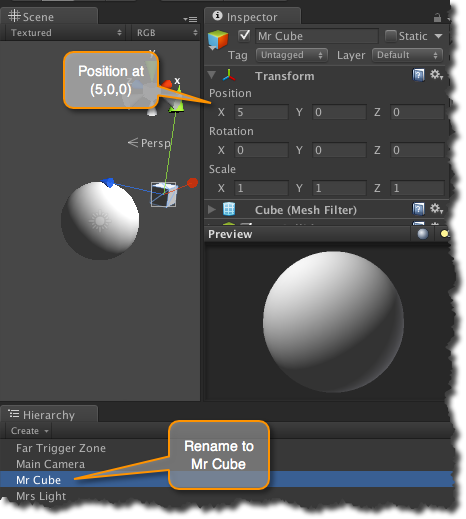
\includegraphics[keepaspectratio,width=\textwidth,height=0.75\textheight]{configure-mr-cube-name-and-position.png}
\caption{Adjusting Name and Position of Mr Cube.}
\label{configure-mr-cube-name-and-position.png}
\end{figure}

\begin{figure}[htbp]
\centering
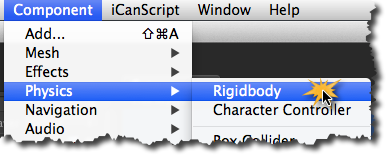
\includegraphics[keepaspectratio,width=\textwidth,height=0.75\textheight]{adding-rigid-body.png}
\caption{Adding a Rigid Body to Mr Cube.}
\label{adding-rigid-body.png}
\end{figure}

\begin{figure}[htbp]
\centering
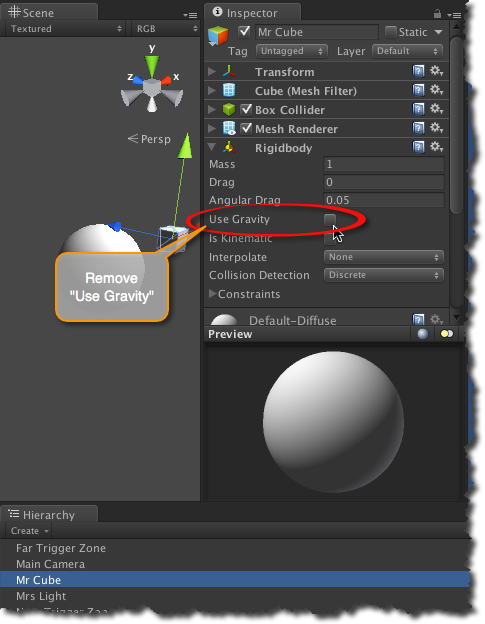
\includegraphics[keepaspectratio,width=\textwidth,height=0.75\textheight]{remove-gravity-from-mr-cube.png}
\caption{Removing gravity from Mr Cube.}
\label{remove-gravity-from-mr-cube.png}
\end{figure}

\section{Hiding the Trigger Zones}
\label{hidingthetriggerzones}

All of our actors are now included in the scene. However, we still need to make one last adjustment: hide the trigger zones.

The trigger zones are the \emph{``magic''} that makes actors change behaviour and everyone knows that \emph{``magic''} must be invisible. So, let's hide those spheres for no one to see. To hide the trigger zones, you need to disable the \emph{Mesh Renderer} as depicted in the below figure.

\begin{figure}[htbp]
\centering
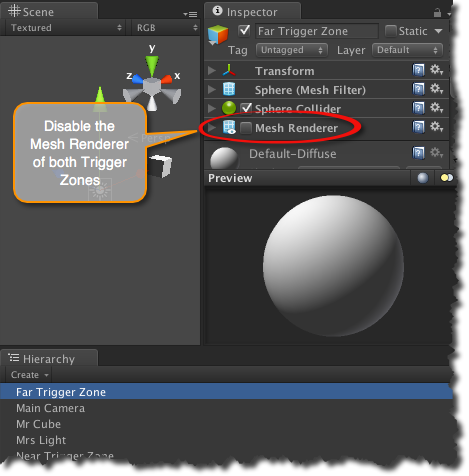
\includegraphics[keepaspectratio,width=\textwidth,height=0.75\textheight]{disable-trigger-zones-mesh-renderer.png}
\caption{Disable the Mesh Renderer of both Trigger Zones.}
\label{disable-trigger-zones-mesh-renderer.png}
\end{figure}
\begin{tipbox}


\includegraphics[width=33pt,height=33pt]{UnityLogo_32x32.png} {\Large \color{black} Unity Tips }

\begin{center}\rule{\textwidth}{0.4pt}\end{center}

\textbf{What's a Renderer?}

\begin{quote}

The \textbf{renderer} is the Unity entity responsible for drawing the scene objects. Each object in a Unity scene includes a renderer component to control its drawing properties. By disabling the \textbf{Mesh Renderer}, you are telling Unity to forgo the drawing of the trigger zones hence hiding them from the user. Hiding the trigger zones does not change the behaviour of other components such as collision detection that is dear to us.
\end{quote}

\end{tipbox}



You are now ready to build your visual scripts!!!

\begin{quote}

(finally you must be saying to yourself).
\end{quote}

\chapter{Opening the iCanScript Editors}
\label{openingtheicanscripteditors}

You are almost ready to create your first visual script. Before you do so, you need to open the following four iCanScript editors:

\begin{itemize}
\item Visual Editor;

\item Library Tree;

\item Hierarchy Tree and;

\item Instance Wizard.

\end{itemize}

All of the editors can be opened for the \begin{color}{blue!70!red}\emph{\textbf{Window->iCanScript->...}}\end{color} menu item. The \emph{Visual Editor} requires a significant screen area so I propose that you combine it with the \emph{Scene} or \emph{Game} window. All of the other editors are narrow and tall and may be combine with the Unity \emph{Project}, \emph{Hierarchy}, or \emph{Inspector} panels.

My preferred window setup for working with iCanScript is:

\begin{itemize}
\item the \emph{\textbf{Visual Editor}} is combined with \emph{Unity's Scene};

\item the \emph{\textbf{Library Tree}} and \emph{\textbf{Hierarchy Tree}} share the bottom section with \emph{Unity's Project} and;

\item the \emph{\textbf{Instance Wizard}} is combined with \emph{Unity's Inspector}.

\end{itemize}

\begin{figure}[htbp]
\centering
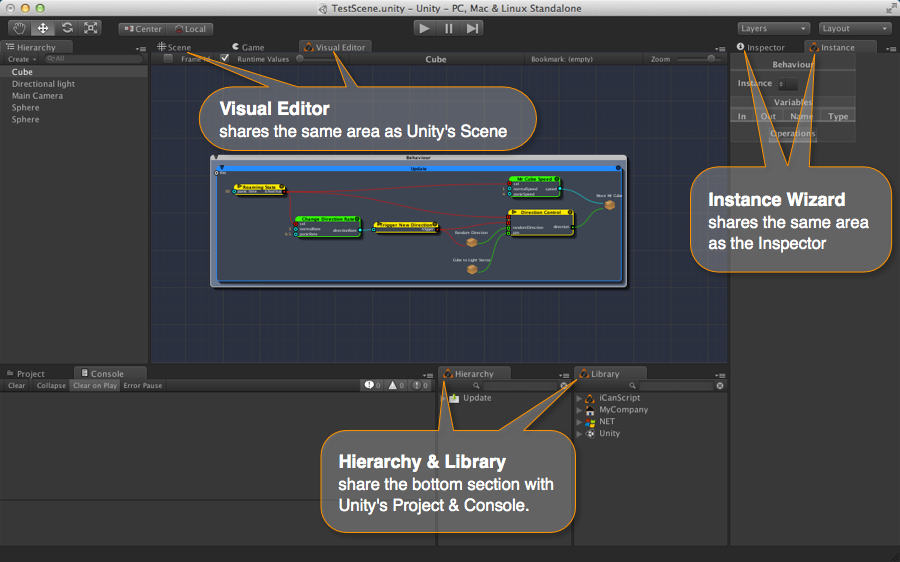
\includegraphics[keepaspectratio,width=\textwidth,height=0.75\textheight]{proposed-icanscript-window-layout.png}
\caption{Proposed iCanScript Window Layout.}
\label{proposed-icanscript-window-layout.png}
\end{figure}

Of course the layout is a matter of taste and you should organize it to your licking (a two screen layout is the best!).

\chapter{Moving Mr Cube (step 1)}
\label{movingmrcubestep1}

Finally, you are ready to write your first visual script. \emph{Mr Cube} movement is ratter complex and shall be implement in phases. In this section, you will create a visual script to move \emph{Mr Cube} at a consistent speed regardless of the performance of the computer or game platform running the script.
\begin{tipbox}


\includegraphics[width=33pt,height=33pt]{Chalkboard-ABCs_32x32.png} {\Large \color{black} What you will learn... }

\begin{center}\rule{\textwidth}{0.4pt}\end{center}

In this section you will learn several key aspects of iCanScript including:

\begin{quote}

\begin{itemize}
\item Adding a visual script to a game object;

\item Defining message handler nodes to process Unity messages;

\item Structuring your visual scripts by encapsulating functionality inside \emph{Package} nodes;

\item Designing logic flows and computations using visual scripts;

\item Using and binding scene objects into your visual scripts;

\item Navigating and extracting entity, variable and function nodes from the iCanScript library.

\end{itemize}
\end{quote}

\end{tipbox}



\section{Installing a Visual Script on \emph{Mr Cube}}
\label{installingavisualscriptonmrcube}

The first step is to install a visual script on \emph{Mr Cube}. This is accomplished by:

\begin{enumerate}
\item Selecting \emph{Mr Cube} in the Hierarchy and;

\item Clicking on the menu item \begin{color}{blue!70!red}\emph{\textbf{Component->iCanScript->Visual Script}}\end{color}.

\end{enumerate}

\begin{figure}[htbp]
\centering
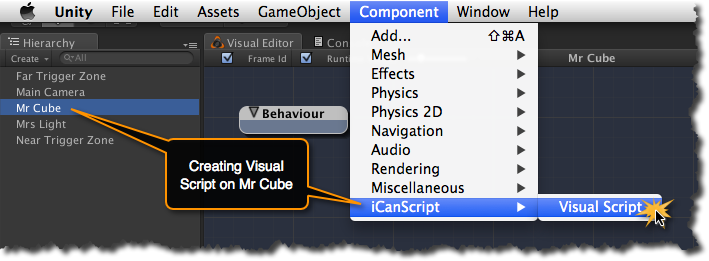
\includegraphics[keepaspectratio,width=\textwidth,height=0.75\textheight]{ics-installing-visual-script-on-mr-cube.png}
\caption{Installing a visual script on \emph{Mr Cube}.}
\label{ics-installing-visual-script-on-mr-cube.png}
\end{figure}

A visual script is now installed on \emph{Mr Cube} and ready to receive Unity messages. To edit the visual script, you must select \emph{Mr Cube} (if not already done) and activate the \emph{Visual Editor} by clicking on its tab.
\begin{tipbox}


\includegraphics[width=33pt,height=33pt]{icanscript-ui-tips_32x32x32.png} {\Large \color{black} iCanScript User Interface Tips }

\begin{center}\rule{\textwidth}{0.4pt}\end{center}

\textbf{Visual Editor :: Centring the visual script (\begin{color}{blue!70!red}\emph{\textbf{Shift-F}}\end{color}):}

\begin{quote}

The hot key \emph{\textbf{Shift-F}} can be used to resize and reposition the visual script in the centre of the viewport. (See the [navigation][] for additional hot keys.)
\end{quote}

\textbf{Scene Editor :: Visualizing which object contains a visual script:}

\begin{quote}

In the Scene editor, iCanScript displays its logo in front of each object that contains a visual script.

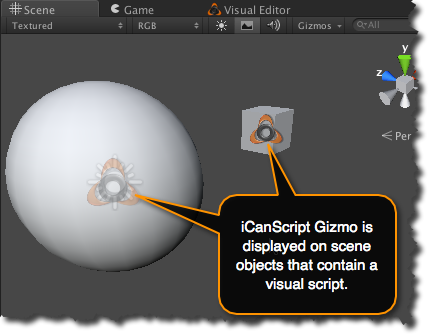
\includegraphics[width=249pt,height=195pt]{ics-gizmo-in-scene.png}
\end{quote}

\textbf{Visual Editor :: Selecting the visual script to edit:}

\begin{quote}

The \emph{\textbf{Visual Editor}} provides a graphical view of the visual script installed on the selected game object. To edit a visual script, you first need to select the game object that contains the visual script.

The name of the game object containing the visual script is displayed in the toolbar of the \emph{Visual Editor}.

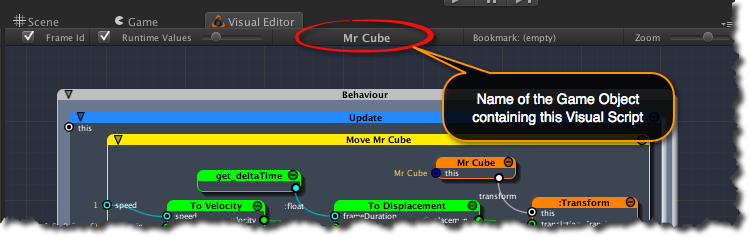
\includegraphics[width=351pt,height=110pt]{name-of-object-including-visual-script.png}

\textbf{Note:} The Visual Editor continues to edit the same visual script (previous selection) if the object selected in the Hierarchy panel does not contain a visual script.
\end{quote}

\end{tipbox}



Currently your visual script contains a single grey node named: \emph{Behaviour}. For iCanScript, the \emph{Behaviour} node is special in two ways:

\begin{itemize}
\item first, it's the top-level node that orchestrates the execution of all visual scripts;

\item secondly, its content is limited to \emph{Message Handler} nodes.

\end{itemize}

Before furthering our example, let's take a moment to examine some of the core constructs of iCanScript:
\begin{tipbox}


\includegraphics[width=33pt,height=33pt]{iCanScriptLogo_32x32x32.png} {\Large \color{black} iCanScript Core Concepts }

\begin{center}\rule{\textwidth}{0.4pt}\end{center}

iCanScript supports two categories of nodes:

\textbf{Action nodes:}

\begin{quote}

\emph{\textbf{Action}} nodes execute functionality created outside the realm of iCanScript. Nodes extracted from libraries and handwriting code are good examples of action nodes.

iCanScript does not have the ability to look inside or alter the functionality underlying \emph{Action} nodes. For iCanScript, \emph{Action} nodes are black-boxes that can be inter-connected, conditionally executed, and packaged to create high-level functionality.
\end{quote}

\textbf{Composite nodes:}

\begin{quote}

\emph{\textbf{Composite}} nodes are used to organize, abstract, and control a subset of the visual script. The subset is embedded, using nesting, inside the composite node creating a parent \slash  child relationship.

A \emph{Composite} node activates its child nodes if the conditions for it own activation are met. For example, a message handler node will execute its internal visual script only when it receives the appropriate message.

Composite nodes exist in several flavours each with distinct behaviour and trigger conditions.
\end{quote}

\end{tipbox}


\begin{tipbox}


\includegraphics[width=33pt,height=33pt]{iCanScriptLogo_32x32x32.png} {\Large \color{black} iCanScript Core Concepts }

\begin{center}\rule{\textwidth}{0.4pt}\end{center}

Every visual script is composed of one \emph{Behaviour} node and one or more \emph{Message Handler} node(s).

\textbf{Behaviour Node:}

\begin{quote}

\emph{\textbf{Behaviour}} is a special composite node that coordinates the execution of the overall visual script. It waits for messages sent from Unity's engine to trigger a subset of the visual script.

The \emph{\textbf{Behaviour}} node uses \emph{\textbf{Message Handler}} nodes to identify which messages the script operates on.

Before creating a visual script, you must first decide which of the Unity messages triggers the execution of your script. A message handler node must be created and embedded in the \emph{Behaviour} node for each message your visual script responds to.
\end{quote}

\begin{tipbox}


\begin{quote}


\includegraphics[width=33pt,height=33pt]{UnityLogo_32x32.png} Details pertaining the available Unity messages are documented in the \emph{MonoBehaviour} section of the \href{http://docs.unity3d.com/Documentation/ScriptReference/MonoBehaviour.html}{Unity Script Reference guide}\footnote{\href{http://docs.unity3d.com/Documentation/ScriptReference/MonoBehaviour.html}{http:/\slash docs.unity3d.com\slash Documentation\slash ScriptReference\slash MonoBehaviour.html}}.
\end{quote}

\end{tipbox}


\textbf{Message Handler Nodes:}

\begin{quote}

A \emph{Message Handler} node is a composite node associated with a specific Unity message. Its purpose is to bridge a Unity message with a subset of your visual script.

When the \emph{Behaviour} node receives a message, it updates the input port values (message parameters) and activates the corresponding \emph{Message Handler} node. The script you create to respond to the message must be embedded in the corresponding \emph{Message Handler} node.
\end{quote}

\end{tipbox}



\section{Installing the \emph{Update} Message Handler}
\label{installingtheupdatemessagehandler}

Before displaying a new frame, Unity sends an \emph{Update} message to each game object in the scene asking them to prepare for the upcoming frame. This \emph{Update} message is ideal to trigger the execution of the visual script to move \emph{Mr Cube}. It gives you the chance to recompute \emph{Mr Cube} position immediately before the scene is displayed.

Your next step is to install the \emph{Update} message handler node whom will serve as the parent trigger for your visual script. The creation of the \emph{Update} message handler node is realized as follows:

1- Right click on the \emph{Behaviour} node to reveal the list of message handlers it supports;
2- Click the \begin{color}{blue!70!red}\emph{\textbf{+ Update}}\end{color} menu item to install the message handler node;

\begin{figure}[htbp]
\centering
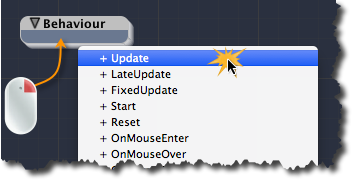
\includegraphics[keepaspectratio,width=\textwidth,height=0.75\textheight]{installing-update-message-handler.png}
\caption{Installing the Update message handler.}
\label{installing-update-message-handler.png}
\end{figure}

A new child node called \emph{Update} is create inside the \emph{Behaviour} node. The \emph{Update} node is blue indicating that it is a message handler. You are now ready to create the visual script to move \emph{Mr Cube} inside the \emph{Update} node.

\section{Visual Script Overview}
\label{visualscriptoverview}

\emph{Mr Cube} visual script will evolve to become somewhat involved as you increase its functionality. To avoid complex and overblown graphs, you should consider structuring the visual script from its inception.

The following diagram depicts the high-level design of the visual script you will create for Mr Cube:

\begin{figure}[htbp]
\centering
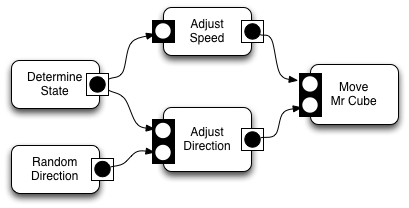
\includegraphics[keepaspectratio,width=\textwidth,height=0.75\textheight]{mr-cube-script-overview.png}
\caption{\emph{Mr Cube} visual script overview.}
\label{mr-cube-script-overview.png}
\end{figure}

It's good practice to segregate and encapsulate functionality into tight bundles and iCanScript has the right \emph{Composite} node to do so: (drum roll{\ldots}) the `\emph{\textbf{Package}}'.

The \emph{Package} is iCanScript most flexible node. It can contain complex graphs and expose only those ports that are made public by the visual script designer. To modify a \emph{Package}, it will need to be \emph{\textbf{unfolded}}, showing its internal graph. Once you have completed its functionality, you may want to \emph{\textbf{fold}} it so that it displays as a singular node or \emph{\textbf{iconize}} it to reduce visual clutter.

The following diagram shows the controls to fold\slash unfold and iconize a \emph{Package} node.

\begin{figure}[htbp]
\centering
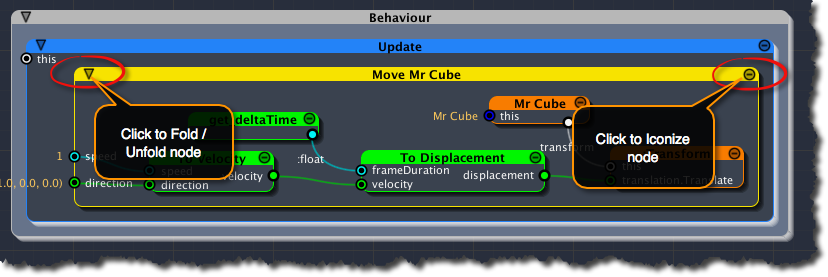
\includegraphics[keepaspectratio,width=\textwidth,height=0.75\textheight]{node-display-state-controls.png}
\caption{Node display state controls.}
\label{node-display-state-controls.png}
\end{figure}

\section{Creating the \emph{``Move Mr Cube Package''}}
\label{creatingthemovemrcubepackage}

Let's create a package to encapsulate the basic movement functionality of \emph{Mr Cube}. This is achieved by:

\begin{itemize}
\item Right clicking on the \emph{Update} node to display the context sensitive menu and;

\item Selecting the \begin{color}{blue!70!red}\emph{\textbf{+ Package}}\end{color} menu item.

\end{itemize}

\begin{figure}[htbp]
\centering
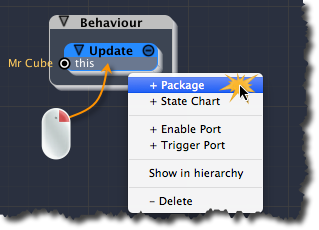
\includegraphics[keepaspectratio,width=\textwidth,height=0.75\textheight]{creating-package-in-update.png}
\caption{Creating the \emph{``Move Mr Cube''} Package.}
\label{creating-package-in-update.png}
\end{figure}

iCanScript adds a package node under the \emph{Update} message handler. By default, the package is yellow and named \emph{``:Package''}. A name that better describes the purpose of the package would be better suited. Do let's rename your new package to: \emph{``Move Mr Cube''}.
\begin{tipbox}


\includegraphics[width=33pt,height=33pt]{icanscript-ui-tips_32x32x32.png} {\Large \color{black} iCanScript User Interface Tips }

\begin{center}\rule{\textwidth}{0.4pt}\end{center}

\textbf{Modifying name of visual elements:}

\begin{quote}

Modifying the node or port name is realized either from the \emph{Inspector} or the iCanScript \emph{Hierarchy Tree}.

The \emph{Inspector} grants detail access to the node or port that is selected in the visual script. It is however limited the selected element only and will require re-selecting if more then one element needs to be modified.

The iCanScript \emph{Hierarchy Tree} offers a tree-like navigation of the entire visual script. It also allows for changing visual element names. In this tutorial, we will always use the \emph{Hierarchy Tree} when modifying node and port names.
\end{quote}

\end{tipbox}



Let's use the \emph{Hierarchy Tree} to change the name of the package.

From the \emph{Visual Editor}, right click on the \emph{:Package} and select the \begin{color}{blue!70!red}\emph{\textbf{Show in hierarchy}}\end{color} menu item (figure \ref{show-package-in-hierarchy.png}). This action displays the selected node in the \emph{Hierarchy Tree}.

\begin{figure}[htbp]
\centering
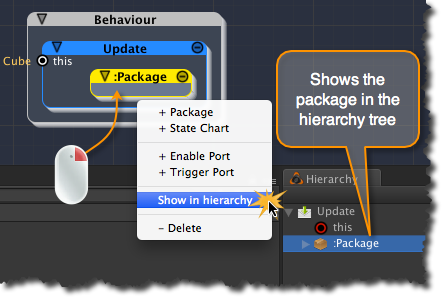
\includegraphics[keepaspectratio,width=\textwidth,height=0.75\textheight]{show-package-in-hierarchy.png}
\caption{Show Package node in iCanScript Hierarchy tree.}
\label{show-package-in-hierarchy.png}
\end{figure}

Double click on the package name in the \emph{Hierarchy Tree} to modify it to \emph{``Move Mr Cube''} (figure \ref{renaming-move-mr-cube-package.png}).
\begin{tipbox}


\includegraphics[width=33pt,height=33pt]{PostitNote_32x32.png} \textbf{Note:} The \emph{Visual Editor} and \emph{Hierarchy Tree} are two views into the visual script. This means that modifications done in the \emph{Hierarchy Tree} are reflected in the \emph{Visual Editor} and vice-versa.

\end{tipbox}



\begin{figure}[htbp]
\centering
\includegraphics[keepaspectratio,width=\textwidth,height=0.75\textheight]{renaming-move-mr-cube-package.png}
\caption{Renaming the package to \emph{Move Mr Cube}.}
\label{renaming-move-mr-cube-package.png}
\end{figure}

\section{Adding \emph{Mr Cube} to the Visual Script}
\label{addingmrcubetothevisualscript}

It's now time to put beef into your hamburger! The first ingredient you need is \emph{Mr Cube}. He can be brought into the visual script by dragging him from Unity's Hierarchy panel into the \emph{Move Mr Cube} package (see figure \ref{drag-and-drop-mr-cube.png}).

\begin{figure}[htbp]
\centering
\includegraphics[keepaspectratio,width=\textwidth,height=0.75\textheight]{drag-and-drop-mr-cube.png}
\caption{Adding Mr Cube to the \emph{Move Mr Cube} package.}
\label{drag-and-drop-mr-cube.png}
\end{figure}

The new \emph{Mr Cube} node is coloured orange indicating that it is an instance of an entity. Factually, \emph{Mr Cube} is an instance of a \emph{Game Object}: a complex entity that contains several components defining its capabilities.
\begin{tipbox}

\includegraphics[width=33pt,height=33pt]{icanscript-ui-tips_32x32x32.png} {\Large \color{black} iCanScript User Interface Tips }

\begin{center}\rule{\textwidth}{0.4pt}\end{center}

\textbf{Instance Nodes and the \emph{Instance Wizard}}
iCanScript includes a dedicated editor called the \emph{Instance Wizard} to manage the variables and operations associated with nodes representing object instances. The \emph{Instance Wizard} is automatically brought forward when such a node is selected.

Using a simple point-and-click interface, the \emph{Instance Wizard} can expose or hide the internal variables and operations of the instance. It is divided in three (3) sections:

\textbf{Instance (top section):}

\begin{quote}

The top section consists of a drop down menu that lists the available functions to create an instance of the proper node type and bind it to the \emph{`this'} port. Since we have dragged in \emph{Mr Cube}, iCanScript has assumed that the instance should be set to the \emph{Mr Cube} game object.
\end{quote}

\textbf{Variables (middle section):}

\begin{quote}

The middle section displays all of the variables (fields \& properties) of the instance. You may expose those variables as input and\slash or output ports by modifying the checkbox on the left of the variable name.
\end{quote}

\textbf{Operations (bottom section):}

\begin{quote}

The bottom section gives access to the operations available for the instance as a list of buttons. Clicking on the operation name exposes that operation on the instance node. Clicking again removes the operation.
\end{quote}

\end{tipbox}



\section{Exposing the \emph{Transform} of \emph{Mr Cube}}
\label{exposingthetransformofmrcube}

In Unity, a game object and its components form a group of inter-related objects. The game object maintains a list of all of its components and each component keeps a reference back to the game object as depicted in figure \ref{game-object-composition.png}.

\begin{figure}[htbp]
\centering
\includegraphics[keepaspectratio,width=\textwidth,height=0.75\textheight]{game-object-composition.png}
\caption{Unity \emph{Game Object} and associated \emph{Components}.}
\label{game-object-composition.png}
\end{figure}

To gain access to a component of the game object, you first need to extract it as a separate instance node. You can then interact with the component variables and operations using the \emph{Instance Wizard}.
\begin{tipbox}

\includegraphics[width=33pt,height=33pt]{UnityLogo_32x32.png} {\Large \color{black} Unity Tips }

\begin{center}\rule{\textwidth}{0.4pt}\end{center}

\begin{quote}

The number and type of components that can be attached to a game object is not limited to the listed displayed in figure 1. The Unity library includes a set of standard components and allows for extending the game object functionality with user defined components.

When you create a visual script on a game object, you are in fact extending that game object by attaching an \emph{iCS\_VisualScript} component to it. iCanScript then uses the iCS\_VisualScript component to edit, compile and run you visual script.
\end{quote}

\end{tipbox}



The component of interest for moving \emph{Mr Cube} is called the \emph{Transform}. It defines the position, rotation, and scale of the game object. Moving \emph{Mr Cube} requires that you change its position hence change its \emph{Transform} component.

Exposing the \emph{Transform} of \emph{Mr Cube} requires that:
1- you reveal the port associated with the \emph{Transform} component and then;
2- extract the transform node to gain access to its variables and operations.

\textbf{\underline{STEP \#1:} Revealing the \emph{transform} port:}

Revealing the \emph{transform} port of \emph{Mr Cube} is a simple matter of:
- selecting the \emph{Mr Cube} node to reveal the \emph{Instance Wizard} (figure \ref{reveal-mr-cube-transform.png});
- clicking the checkbox on the left side of the \emph{``transform''} variable in the \emph{Instance Wizard} (you may need to scroll to the bottom of the \emph{Variables} section).

\begin{figure}[htbp]
\centering
\includegraphics[keepaspectratio,width=\textwidth,height=0.75\textheight]{reveal-mr-cube-transform.png}
\caption{Reveal Mr Cube transform port.}
\label{reveal-mr-cube-transform.png}
\end{figure}

\textbf{\underline{STEP \#2:} Extracting the \emph{transform} instance node:}

The next step is to extract the transform node from \emph{Mr Cube}. The good news is that iCanScript includes a feature that automatically creates an instance node when you drag a port into an empty area.

Since the \emph{Move Mr Cube} package tightly surrounds the \emph{Mr Cube} node, dragging the port into an empty area inside the \emph{Move Mr Cube} node may be challenging (Undo can be used if mistakes are made). In the current situation, the easiest way is to drag the \emph{transform} port up towards the title bar of the \emph{Move Mr Cube} node and release it their (see figure \ref{extract-mr-cube-transform.png}).

You can later reposition the new transform node by dragging it from its title bar. Likewise, you can relocate the ports by sliding them on the boundaries of the node. 

\begin{figure}[htbp]
\centering
\includegraphics[keepaspectratio,width=\textwidth,height=0.75\textheight]{extract-mr-cube-transform.png}
\caption{Extract Mr Cube transform.}
\label{extract-mr-cube-transform.png}
\end{figure}
\begin{tipbox}

\includegraphics[width=33pt,height=33pt]{UnityLogo_32x32.png} {\Large \color{black} Unity Tips }

\begin{center}\rule{\textwidth}{0.4pt}\end{center}

\textbf{Game Object Transform:}

\begin{quote}

Every \emph{Game Object} in Unity includes a \emph{Transform} component. The \emph{Transform} component defines the position, rotation, and scale of the object with respect to its parent. If no parent exists, then the \emph{Transform} is considered global -- relative to the world coordinates -- as for all actors in our example.
\end{quote}

\end{tipbox}



\section{Adding the \emph{Translation} operation to the \emph{Transform} node}
\label{addingthetranslationoperationtothetransformnode}

Now that you have access to the \emph{Transform} instance node, you can select it and browse its variables and operations using the \emph{Instance Wizard} (figure \ref{add-mr-cube-translation.png}).

If you browse the \emph{Operations} section, you will find that the \emph{Transform} node includes several \emph{Translate({\ldots})} operations that can be used to move \emph{Mr Cube}. We are interested in the \emph{Translate} operation that utilizes a \emph{Vector3} type for the displacement.

To add the \emph{Translate} operation to your visual script, you will need to depress the \begin{color}{blue!70!red}\emph{\textbf{Translate(translation:Vector3)}}\end{color} button of the \emph{Instance Wizard}. Once the operation is added, its button is shown as depressed and the text as bolded. Clicking the button a second time will remove the operation from the visual script. Make certain that the \emph{Translate} operation is added before moving on.

\begin{figure}[htbp]
\centering
\includegraphics[keepaspectratio,width=\textwidth,height=0.75\textheight]{add-mr-cube-translation.png}
\caption{Add Mr Cube translation operation.}
\label{add-mr-cube-translation.png}
\end{figure}

With the \emph{Translate} operation added, you'll notice a new port named \emph{``translation.Translate''} appearing on the \emph{Transform} node. As you may have guessed, this new input port configures the translation to be applied by the \emph{Translate} operation.

The default value for the translation is (0,0,0). You will learn to create a visual script to dynamically change the translation value in the sections to follow. 

\section{Moving with Consistent Velocity}
\label{movingwithconsistentvelocity}

Your next task is to feed a displacement value to the \emph{Translate} operation of \emph{Mr Cube}. While this seams easy, it does present a challenge{\ldots}

\textbf{The Challenge:}
The problem is that the displacement is applied for each frame and that the frame rate (\# of frames \slash  second) is dependent on the performance of the computer or gaming platform. This means that if the same displacement value is applied, \emph{Mr Cube} will move lightning fast on high-end gaming computers and turtle slow on entry level portable devices.

\textbf{The Solution:}
To maintain constant velocity on all platform regardless of their performance, you need to adjust the magnitude of the displacement according to the frame rate. So how do you do that?

As starters, you need to control the velocity of \emph{Mr Cube} and derive the displacement from it. The displacement is computed by equation \#1:
\begin{tipbox}

\textbf{Eq. \#1. Calculation of the displacement for a frame}

\begin{verbatim}
displacement= velocity * frame_duration;
\end{verbatim}

\end{tipbox}



The result of this equation is that higher the frame rate, smaller are the displacement values added to the movement for each frame. Therefore, the velocity is maintained irrespectively of the computing performance.

From equation 1, you need to bring in play an operator that multiplies the velocity (a \emph{Vector3} value) and the frame duration (a \emph{scalar} value).

Using the search field in the iCanScript library, type the characters \emph{``mul''} to reveal the available multiply operators. Drag the multiply operation under the \emph{Vector3} type into the \emph{Move Mr Cube} package as depicted in figure \ref{adding-velocity-to-displacement-node.png}.

\begin{figure}[htbp]
\centering
\includegraphics[keepaspectratio,width=\textwidth,height=0.75\textheight]{adding-velocity-to-displacement-node.png}
\caption{Adding a function to convert velocity into displacement.}
\label{adding-velocity-to-displacement-node.png}
\end{figure}

The \emph{``op\_Multiply''} node is coloured green indicating that it is a function. Functions are created outside iCanScript and imported into the iCanScript library. In this particular case, the multiply operator is a member function of the \emph{Vector3} class that is part of the Unity Engine library (the hierarchy in the \emph{Library Tree} is reminiscence of this structure).

The new node is created with generic names. To improve on the clarity of the visual script, you should rename the node and its ports to reflect the intended functionality.

Follow these steps to rename the \emph{op\_Multiply} node:

\begin{enumerate}
\item Right click on the \emph{``op\_Multiply''} node to bring up the context menu;

\item Select the \emph{Show in Hierarchy} menu item;

\item From the hierarchy tree, unfold the node and rename it and its ports as depicted in figure \ref{renaming-to-displacement-node.png}.

\end{enumerate}
\begin{tipbox}

\includegraphics[width=33pt,height=33pt]{icanscript-ui-tips_32x32x32.png} {\Large \color{black} iCanScript User Interface Tips }

\begin{center}\rule{\textwidth}{0.4pt}\end{center}

\begin{quote}

You need to double click on the name in the hierarchy tree to edit it.
\end{quote}

\end{tipbox}



\begin{figure}[htbp]
\centering
\includegraphics[keepaspectratio,width=\textwidth,height=0.75\textheight]{renaming-to-displacement-node.png}
\caption{Renaming the node that converts the velocity to a displacement.}
\label{renaming-to-displacement-node.png}
\end{figure}

The next step is to bind the \emph{displacement} output port of the \emph{To Displacement} node to the \emph{translation} input port on the \emph{Transform} node. This is super simple to accomplish: just drag the \emph{``displacement''} port onto the \emph{``translation.Translate''} port and {\ldots} Voilà! it's done. Now the computed displacement changes the position of \emph{Mr Cube} on every frame.

\begin{figure}[htbp]
\centering
\includegraphics[keepaspectratio,width=\textwidth,height=0.75\textheight]{bind-displacement-to-translation.png}
\caption{Bind the computed displacement to Mr Cube transform.}
\label{bind-displacement-to-translation.png}
\end{figure}

You are still missing the frame duration value. Unity has us covered with that. The \emph{Time} type supports several time related functions. The duration of the last executed frame is held in a variable named \emph{deltaTime}.

Start typing \emph{``delta''} in the search field of the \emph{Library} panel to expose the \emph{deltaTime} variable. You should see it under the \emph{Time} type of the UnityEngine section.

Drag it from the library into the \emph{Move Mr Cube} package and bind its output (named \emph{:float}) to the \emph{frameDuration} input of the \emph{To Displacement} node. The final result should look like figure \ref{adding-delta-time.png}.

\begin{figure}[htbp]
\centering
\includegraphics[keepaspectratio,width=\textwidth,height=0.75\textheight]{adding-delta-time.png}
\caption{Adding frame duration for displacement computation.}
\label{adding-delta-time.png}
\end{figure}
\begin{tipbox}

\includegraphics[width=33pt,height=33pt]{UnityLogo_32x32.png} {\Large \color{black} Unity Tips }

\begin{center}\rule{\textwidth}{0.4pt}\end{center}

\textbf{The \emph{CharacterController} component:}

\begin{quote}

Advised users of Unity will have noticed that we have reproduced the functionality to move a game object using relative speed; a functionality that is available in the \emph{CharacterController} component.

We have deliberately avoided the \emph{CharacterController} to focus the learning experience on building visual scripts. The \emph{CharacterController} offers many features that are beyond the scope of this tutorial. We strongly advise that you take some time to learn about the \emph{CharacterController} before building large on complex projects with Unity.
\end{quote}

\end{tipbox}



\section{Controlling Speed and Direction Separately}
\label{controllingspeedanddirectionseparately}

Referencing back to the overview of the visual script (\autoref{visualscriptoverview}) depicted in figure \ref{mr-cube-script-overview.png}, you will notice that the \emph{Move Mr Cube} package receives its input values from the \emph{Adjust Direction} \& \emph{Adjust Speed} packages (you will build these packages later on). This means that separate controls for direction and speed are required.

Your next task is to extend your visual script to:

\begin{itemize}
\item accept two (2) inputs: a \emph{direction} and a \emph{speed} value;

\item compute the velocity value from the \emph{direction} and \emph{speed} inputs;

\item bind the ``computed velocity'' to the \emph{velocity} input of the \emph{To Displacement} node created in the previous section.

\end{itemize}

In our example, the \emph{speed} and \emph{direction} are defined as:

\begin{itemize}
\item the distance travel in one (1) second and;

\item a unit vector pointing in the direction of movement;

\end{itemize}

respectively.

From these definitions, you can calculate the velocity by scaling the direction vector (a unit vector) by the speed (a scale value) as described in equation \#2:
\begin{tipbox}

\textbf{Eq. \#2. Calculation of the velocity.}

\begin{verbatim}
velocity = speed * direction
\end{verbatim}

\end{tipbox}


\begin{tipbox}

\includegraphics[width=33pt,height=33pt]{PostitNote_32x32.png} \textbf{Note:} A \emph{unit vector} is a vector who's length is equal to one (1).

\end{tipbox}



Equation \#2 has exactly the same structure as the displacement calculation performed in the previous section: you need to multiply a vector value and a scaler value. This is your chance at trying another cool feature of iCanScript: \textbf{node cloning} (without social or legal issues!!!).

To clone the multiply operator, you need to press the \begin{color}{blue!70!red}\emph{\textbf{Shift}}\end{color} key and drag the \emph{To Displacement} node in an empty area inside the \emph{Move Mr Cube} package (see figure \ref{duplicate-vector-scale.png}).

\begin{figure}[htbp]
\centering
\includegraphics[keepaspectratio,width=\textwidth,height=0.75\textheight]{duplicate-vector-scale.png}
\caption{Duplicating the vector scale node.}
\label{duplicate-vector-scale.png}
\end{figure}

Once more, you should rename the node and ports to better describe the intent. Use the \emph{Hierarchy Tree} as you have done for the \emph{To Displacement} node to rename the new node and its ports as shown in figure \ref{rename-to-velocity-node.png}.

You also need to bind the \emph{velocity} output port of the new \emph{To Velocity} node to the \emph{velocity} input port of the \emph{To Displacement} node.

\begin{figure}[htbp]
\centering
\includegraphics[keepaspectratio,width=\textwidth,height=0.75\textheight]{rename-to-velocity-node.png}
\caption{Properly rename the ``To Velocity'' node.}
\label{rename-to-velocity-node.png}
\end{figure}

\section{Publishing the Interface}
\label{publishingtheinterface}

Now you have completed the functionality of the \emph{Move Mr Cube} package. The last step is to publish the \emph{speed} and \emph{direction} ports so that they can be accessed from outside the \emph{Move Mr Cube} package. This is easily done by dragging them on the left edge of the \emph{Move Mr Cube} package. The final build of the \emph{Move Mr Cube} package can be seen in figure \ref{publish-speed-and-direction.png}.

\begin{figure}[htbp]
\centering
\includegraphics[keepaspectratio,width=\textwidth,height=0.75\textheight]{publish-speed-and-direction.png}
\caption{Publish speed and direction ports.}
\label{publish-speed-and-direction.png}
\end{figure}

\section{Running the \emph{Move Mr Cube} Visual Script}
\label{runningthemovemrcubevisualscript}

I bet your fingers are twitching to give your new script a go.

Before you do so, you need to configure initial values for the \emph{speed} and \emph{direction} ports. The initial values are configured using the \emph{Inspector}.

Make certain that the \emph{Mr Cube} game object is selected and open the \emph{Inspector}. You will see that a \emph{visual script component} is installed on \emph{Mr Cube}. Unfold the \emph{visual script component} and you will see that it contains two sections:

\begin{itemize}
\item a \emph{\textbf{Selected Object}} section and;

\item an \emph{\textbf{Engine Selected Object}} section.

\end{itemize}

You will be using the \emph{Selected Object} section to configure the \emph{``speed''} and \emph{``direction''} ports. Unfold the \emph{Selected Object} section if it is folded.

With the \emph{Inspector} open, select the \emph{speed} port in the visual editor. You will see the details of the port presented in the visual script component. Change the speed value from zero (0) to one (1).

Now select the \emph{direction} port in the visual editor. The \emph{Inspector} information will change to match your new selection. Change the \emph{direction} value from (0,0,0) to (--1,0,0).

You are all done; the initial values are now configured.

\begin{figure}[htbp]
\centering
\includegraphics[keepaspectratio,width=\textwidth,height=0.75\textheight]{change-speed-value.png}
\caption{Change speed to 1.}
\label{change-speed-value.png}
\end{figure}

\begin{figure}[htbp]
\centering
\includegraphics[keepaspectratio,width=\textwidth,height=0.75\textheight]{change-direction-value.png}
\caption{Change direction to (--1,0,0).}
\label{change-direction-value.png}
\end{figure}

Hit the run button at the top of the Unity editor to give it a whirl (yeh!!!).

iCanScript compiles and runs your script. \emph{Mr Cube} will start moving towards the centre of the scene (0,0,0) and continues forever in the same direction.

You can configure different values of direction and speed while your script is running. The new values are immediately impacting the behaviour of your script. However, the values configured while the engine is running are temporary and they will revert back to their initial configured values once the Unity game engine is stopped.
\begin{tipbox}

\includegraphics[width=33pt,height=33pt]{icanscript-ui-tips_32x32x32.png} {\Large \color{black} iCanScript User Interface Tips }

\begin{center}\rule{\textwidth}{0.4pt}\end{center}

The details of the selected node or port are accessible from the visual script component in the \emph{Inspector}. The visual script component inspector is divided in two sections:

\textbf{Selected Object:}

\begin{quote}

This section allows to view and configure the attributes of the selected node or port.
\end{quote}

\textbf{Selected Engine Object:}

\begin{quote}

This section displays in-depth information to help debug the visual script. This information will not be used in this tutorial.
\end{quote}

\end{tipbox}



\section{Accessing Runtime Information}
\label{accessingruntimeinformation}

Let's take this opportunity to discuss some of the basic debugging features of iCanScript.

The visual editor remains active while the script is running. Selecting the visual editor tab will bring it forward. You may decide to relocate it so that both the visual editor and the game window be visible. 

\begin{figure}[htbp]
\centering
\includegraphics[keepaspectratio,width=\textwidth,height=0.75\textheight]{runtime-display.png}
\caption{iCanScript Visual Editor with runtime debug information.}
\label{runtime-display.png}
\end{figure}

The visual editor displays the following runtime information in the centre of it's toolbar:

\begin{itemize}
\item the current frame \#;

\item the average frame rate (in frames \slash  sec).

\end{itemize}

In addition, the Visual Editor toolbar includes several options to control the display of runtime information. These options are:

\textbf{Enable\slash Disable display of the frame \#}
 : Enable this control to display the last executed frame \# in the title bar of each node. The display of the last executed frame \# is especially useful when conditional execution is used. It helps differentiate the nodes that are executing from the nodes that are stalled.

\textbf{Enable\slash Disable display of port values}
 : Enable this control to display the runtime values of the ports. The runtime values are displayed in beige and are periodically refreshed.

\textbf{Slider to control the refresh period}
 : This slider is used to control the frequency at which the runtime information is displayed in the visual editor. Depending on the performance of your computer, the display of runtime information could impair on the frame rate of your game. Reducing the refresh rate of the runtime information will reduce the performance impact on your game.

\section{Recap on Your First Visual Script}
\label{recaponyourfirstvisualscript}

So what have you done so far? You have:

\begin{itemize}
\item Create the Unity scene to host your example project;

\item Installed a visual script on the \emph{Mr Cube} game object;

\item Created the \emph{Update} message handler to contain and execute your visual script on each frame;

\item Created a package to encapsulate the script to control the movement of \emph{Mr Cube} using speed and direction;

\item Dragged the \emph{Mr Cube} game object inside the script and extracted its \emph{Transform} component;

\item Build a small equation to translate the speed and direction inputs into a displacement to be applied on \emph{Mr Cube} transform;

\item Publish the \emph{speed} \& \emph{direction} ports onto the \emph{Move Mr Cube} package for easy access by other packages.

\item Tested your new script with predefined speed \& direction values.

\end{itemize}

\chapter{Enabling \& Disabling Ms Light}
\label{enablingdisablingmslight}

\begin{tipbox}


{\Large \color{black} To Be Continued ... }

\end{tipbox}


\chapter{Homing on Ms Light}
\label{homingonmslight}

\begin{tipbox}


{\Large \color{black} To Be Continued ... }

\end{tipbox}


\chapter{Creating a Timer Utility}
\label{creatingatimerutility}

\begin{tipbox}


{\Large \color{black} To Be Continued ... }

\end{tipbox}


\chapter{Changing Direction}
\label{changingdirection}

\begin{tipbox}


{\Large \color{black} To Be Continued ... }

\end{tipbox}


\chapter{Mr Cube Roaming State}
\label{mrcuberoamingstate}

\begin{tipbox}


{\Large \color{black} To Be Continued ... }

\end{tipbox}


\chapter{Adding a Panic State}
\label{addingapanicstate}

\begin{tipbox}


{\Large \color{black} To Be Continued ... }

\end{tipbox}


\chapter{Beautifying your Scripts}
\label{beautifyingyourscripts}

\begin{tipbox}


{\Large \color{black} To Be Continued ... }

\end{tipbox}


\pagebreak 

\part{User Interface}
\label{userinterface}

\chapter{Menus}
\label{menus}

iCanScript installs itself in Unity's Edit, Component, Windows and Help menus. This section describes the iCanScript functionality associated with each menu item.

\section{Edit Menu}
\label{editmenu}

iCanScript extends Unity's \begin{color}{blue!70!red}\emph{\textbf{Edit}}\end{color} menu with navigation features and the ability to create a Visual script as depicted in the below figure.

\begin{figure}[htbp]
\centering
\includegraphics[keepaspectratio,width=\textwidth,height=0.75\textheight]{ics-menu-edit.png}
\caption{iCanScript Edit menu extension.}
\label{ics-menu-edit.png}
\end{figure}

\subsection{Edit-$>$iCanScript-$>$Create Visual Script}
\label{edit-icanscript-createvisualscript}

\emph{\textbf{Summary:}}

\begin{verbatim}
    Attaches a visual script component to the selected game object.
\end{verbatim}

\emph{\textbf{Description:}}

The \begin{color}{blue!70!red}\emph{\textbf{Create Visual Script}}\end{color} menu item is used to attach an iCanScript Visual Script component to the selected game object.

The Visual Script component is at the root of your visual script. It includes the iCanScript engine code that compiles and runs the visual script when the Unity engine runs. It also saves \& reloads your visual script when the scene in which it is contained is saved or reloaded.

A game object containing an iCanScript Visual Script can be edited using the visual editor.

\begin{table}[htbp]
\begin{minipage}{\linewidth}
\setlength{\tymax}{0.5\linewidth}
\centering
\small
\caption{Create Visual Script Enable State}
\label{createvisualscriptenablestate}
\begin{tabulary}{\textwidth}{@{}CL@{}} \toprule
Menu State&Condition\\
\midrule
\emph{\textbf{Enabled}}&- Selected game object without a Visual Script component.\\
\emph{\textbf{Disabled}}&- No selected object;- Selected object already has a Visual Script component.\\

\bottomrule

\end{tabulary}
\end{minipage}
\end{table}

\subsection{Edit-$>$iCanScript-$>$Center Visual Script}
\label{edit-icanscript-centervisualscript}

\emph{\textbf{Summary:}}

\begin{verbatim}
    Centres the visual script in the viewport.
\end{verbatim}

\emph{\textbf{Description:}}

The \begin{color}{blue!70!red}\emph{\textbf{Center Visual Script}}\end{color} menu item is used to reposition the visual script in the centre of the visual editor viewport.

The zoom factor of the viewport may be adjusted to improve visual script visibility.

\subsection{Edit-$>$iCanScript-$>$Center Selected}
\label{edit-icanscript-centerselected}

\emph{\textbf{Summary:}}

\begin{verbatim}
    Centres the selected node / port in the viewport.
\end{verbatim}

\emph{\textbf{Description:}}

The \begin{color}{blue!70!red}\emph{\textbf{Center Selected}}\end{color} menu item is used to reposition the selected node in the centre of the visual editor viewport.

The zoom factor of the viewport may be adjusted to improve selected node visibility.

\section{Component Menus}
\label{componentmenus}

Creating a visual script with iCanScript requires that you install the iCanScript Visual Script component on your game object. The iCanScript Visual Script component can be attached using Unity's top-level \emph{Component} menu as well as the \emph{Add Component} button located in the Inspector.

\begin{figure}[htbp]
\centering
\includegraphics[keepaspectratio,width=\textwidth,height=0.75\textheight]{menu-component.png}
\caption{iCanScript Component menu extension.}
\label{menu-component.png}
\end{figure}

\begin{figure}[htbp]
\centering
\includegraphics[keepaspectratio,width=\textwidth,height=0.75\textheight]{menu-component2.png}
\caption{iCanScript Inspector-$>$Component menu extension.}
\label{menu-component2.png}
\end{figure}

\subsection{Attaching a Visual Script component}
\label{attachingavisualscriptcomponent}

The \begin{color}{blue!70!red}\emph{\textbf{Create Visual Script}}\end{color} menu item is used to attach an iCanScript Visual Script component to the selected game object.

The Visual Script component is at the root of your visual script. It includes the iCanScript engine code that compiles and runs the visual script when the Unity engine runs. It also saves \& reloads your visual script when the scene in which it is contained is saved or reloaded.

A game object containing an iCanScript Visual Script can be edited using the visual editor.

\begin{table}[htbp]
\begin{minipage}{\linewidth}
\setlength{\tymax}{0.5\linewidth}
\centering
\small
\caption{Create Visual Script Enable State}
\label{createvisualscriptenablestate}
\begin{tabulary}{\textwidth}{@{}CL@{}} \toprule
Menu State&Condition\\
\midrule
\emph{\textbf{Enabled}}&- Selected game object without a Visual Script component.\\
\emph{\textbf{Disabled}}&- No selected object;- Selected object already has a Visual Script component.\\

\bottomrule

\end{tabulary}
\end{minipage}
\end{table}

\section{Window Menu}
\label{windowmenu}

iCanScript installs menu items to open its five (5) editors \& panels in Unity's top-level \emph{Window} menu.

\begin{figure}[htbp]
\centering
\includegraphics[keepaspectratio,width=\textwidth,height=0.75\textheight]{menu-window.png}
\caption{iCanscript Window menu extension.}
\label{menu-window.png}
\end{figure}

\subsection{Window-$>$iCanScript-$>$Preferences}
\label{window-icanscript-preferences}

\emph{\textbf{Summary:}}

\begin{verbatim}
    Opens the Preferences Panel
\end{verbatim}

\emph{\textbf{Description:}}

iCanScript \begin{color}{blue!70!red}\emph{\textbf{Preference Panel}}\end{color} is used to configure the appearance and global behaviour of iCanScript editors \& panels.

The iCanScript preference configuration is save for the current user session and is independent of visual script saved data.

The Preference Panel also includes iCanScript version information.

\subsection{Window-$>$iCanScript-$>$Visual Editor}
\label{window-icanscript-visualeditor}

\emph{\textbf{Summary:}}

\begin{verbatim}
    Opens the Visual Editor.
\end{verbatim}

\emph{\textbf{Description:}}

The Visual Editor is the core editor of iCanScript. It is where you will create and modify your visual scripts.

The Visual Editor displays the visual script associated with the currently selected game object. The visual editor will be empty if no game object is selected or the selected game object does not include an iCanScript Behaviour component.

\subsection{Window-$>$iCanScript-$>$Hierarchy}
\label{window-icanscript-hierarchy}

\emph{\textbf{Summary:}}

\begin{verbatim}
    Opens the visual script hierarchy tree.
\end{verbatim}

\emph{\textbf{Description:}}

The Hierarchy Tree Editor is used to navigate and edit your visual script as a tree view. It complements the graphical visual editor.

You can edit the node \& port names and quickly navigate your visual script from the hierarchy tree editor.

\subsection{Window-$>$iCanScript-$>$Library}
\label{window-icanscript-library}

\emph{\textbf{Summary:}}

\begin{verbatim}
    Opens the node library tree.
\end{verbatim}

\emph{\textbf{Description:}}

The \emph{\textbf{Library Panel}} is a repository of all available nodes that can be dragged into your visual script. It includes Unity's core library, iCanScript base node library as well as some of the .NET functionality.

The Library Panel can easily be extended with your own nodes. Refer to section Extending iCanScript to learn how to add your own nodes in the library.

\subsection{Window-$>$iCanScript-$>$Instance Wizard}
\label{window-icanscript-instancewizard}

\emph{\textbf{Summary:}}

\begin{verbatim}
    Opens the node instance wizard.
\end{verbatim}

\emph{\textbf{Description:}}

The \emph{\textbf{Instance Wizard}} is used to intelligently present and configure the fields, properties, and functions associated to the type of a node in your visual script.

The instance wizard will automatically activate when selecting a node associate with a specific type (i.e. .NET class).

\section{Help Menu}
\label{helpmenu}

iCanScript extends Unity's \begin{color}{blue!70!red}\emph{\textbf{Help}}\end{color} menu to provide quick access to the product web site, documentation and support pages.

\begin{figure}[htbp]
\centering
\includegraphics[keepaspectratio,width=\textwidth,height=0.75\textheight]{ics-menu-help.png}
\caption{iCanScript Help menu extension.}
\label{ics-menu-help.png}
\end{figure}

\subsection{Help-$>$iCanScript-$>$Home Page}
\label{help-icanscript-homepage}

\emph{\textbf{Summary:}}

\begin{verbatim}
    Opens iCanScript home page in the default Web browser.
\end{verbatim}

\emph{\textbf{Description:}}

The \begin{color}{blue!70!red}\emph{\textbf{Home Page}}\end{color} menu item is used to open the home page of the iCanScript Web site in a new internet browser window.

An internet connection is required to access the iCanScript home page.

\subsection{Help-$>$iCanScript-$>$User's Guide}
\label{help-icanscript-usersguide}

\emph{\textbf{Summary:}}

\begin{verbatim}
    Opens iCanScript user manual in the default Web browser.
\end{verbatim}

\emph{\textbf{Description:}}

The \begin{color}{blue!70!red}\emph{\textbf{User's Guide}}\end{color} menu item is used to open the iCanScript online user guide in a new internet browser window.

An internet connection is required to access the iCanScript online user guide.

\subsection{Help-$>$iCanScript-$>$Release Notes}
\label{help-icanscript-releasenotes}

\emph{\textbf{Summary:}}

\begin{verbatim}
    Opens latest release notes in the default Web browser.
\end{verbatim}

\emph{\textbf{Description:}}

The \begin{color}{blue!70!red}\emph{\textbf{Release Notes}}\end{color} menu item is used to open the iCanScript latest release information in a new internet browser window.

The release notes are sorted from the latest release to the oldest release for your convenience. A copy of the release notes in PDF format can also be downloaded from the web site.

An internet connection is required to access the iCanScript release note pages.

\subsection{Help-$>$iCanScript-$>$Customer Request}
\label{help-icanscript-customerrequest}

\emph{\textbf{Summary:}}

\begin{verbatim}
    Opens the feature request and bug report form.
\end{verbatim}

\emph{\textbf{Description:}}

The \begin{color}{blue!70!red}\emph{\textbf{Customer Request}}\end{color} menu item is used to submit feature requests and bug reports for the iCanScript product. You can also browse the status of existing customer requests.

The customer request form is Web based and requires an active internet connection.

\subsection{Help-$>$iCanScript-$>$Check for Updates{\ldots}}
\label{help-icanscript-checkforupdates}

\emph{\textbf{Summary:}}

\begin{verbatim}
    Validates the current version against latest available release.
\end{verbatim}

\emph{\textbf{Description:}}

The \begin{color}{blue!70!red}\emph{\textbf{Check for Update}}\end{color} menu item is used to determine if you have the latest official release of iCanScript. You will be prompted to download the latest version if your version is out-of-date.

Validation of the latest iCanScript version requires an active internet connection.

\pagebreak 

\part{Extending iCanScript}
\label{extendingicanscript}

\chapter{Extending iCanScript}
\label{extendingicanscript}

From its inception, iCanScript was designed to be extendable with the addition of user defined nodes. Once installed, the user defined nodes are accessible from the [Library Tree].

Extending the iCanScript library is realized by:

\begin{enumerate}
\item Tagging your Source Code (\autoref{taggingyoursourcecode});

\item Importing Public Members (\autoref{importingpublicmembers});

\item Adding Message Handlers (\autoref{addingmessagehandlers}).

\end{enumerate}

The following picture illustrates how the iCanScript library gets populated and used. You are given three access points (purple) to include your own packages and nodes inside the iCanScript library. The iCanScript library gets repopulated for every recompile of the Unity scripts.

\begin{figure}[htbp]
\centering
\includegraphics[width=479pt,height=295pt]{extending-node-information-flow.png}
\caption{iCanScript library information flow.}
\label{extending-node-information-flow.png}
\end{figure}

\includegraphics[width=32pt,height=30pt]{stamp-1-purple.png} \textbf{Tagged Source Code:} You can add to the iCanScript library by tagging your source code with specialized .NET attributes. This provides for fine control of which elements in your source code are published to the iCanScript user.

\includegraphics[width=32pt,height=30pt]{stamp-2-purple.png} \textbf{Importing Public Members:} You can add to the iCanScript library by batch importing all \emph{public} members of specified programatic types. This method is specially useful for importing libraries for which you do not have the source code.

\includegraphics[width=32pt,height=30pt]{stamp-3-purple.png} \textbf{Message Installation:} The .NET reflection technology allows for dynamic messaging; a technic used to dynamically invoke a functionality only if it is defined for a software object. A script responds to dynamic messages if it includes the appropriate message handlers. You can populate the iCanScript library with the signature of message handlers for given programatic types. Afterward, the signature can be used by the iCanScript user to build the message handler nodes.

\includegraphics[width=32pt,height=30pt]{stamp-4-orange.png}\includegraphics[width=32pt,height=30pt]{stamp-5-orange.png} The iCanScript editors extracts from the library node and port information when building the visual script. The visual script manifest and layout information is saved along with the game object that includes the \emph{iCS\_VisualScript} component.

\includegraphics[width=32pt,height=30pt]{stamp-6-orange.png} iCanScript also generates the \emph{iCS\_Behaviour} code that is needed by Unity to execute the the Visual Script. The behaviour code includes:

\begin{enumerate}
\item the message handlers;

\item the control logic that determine the execution order of nodes, and;

\item the nodes converted into .NET code.

\end{enumerate}

\includegraphics[width=32pt,height=30pt]{stamp-7-orange.png}When the Unity engine is ran, the iCS\_Behaviour code instantiates the variables, invokes the .NET code of the nodes, and responds to the message handlers. The iCanScript core executive (iCanScriptEngine.dll) assures the execution order and resolves data contention.

\chapter{Tagging your Source Code}
\label{taggingyoursourcecode}

iCanScript includes several .NET attributes to control which part of your source code is to be included in the iCanScript library. These attributes enables fine control over which fields, properties and functions become visible to the iCanScript user.

iCanScript scans the .NET assemblies to populate its library with public classes tagged with the \emph{iCS\_Class} attribute. The assembly scan is performed after every recompile of the Unity scripts.

The following table depicts the mapping between C\# source code and iCanScript objects:

\begin{table}[htbp]
\begin{minipage}{\linewidth}
\setlength{\tymax}{0.5\linewidth}
\centering
\small
\caption{Mapping between C\# source code and iCanScript objects.}
\label{mappingbetweencsourcecodeandicanscriptobjects.}
\begin{tabulary}{\textwidth}{@{}LCL@{}} \toprule
Source Code&\multicolumn{2}{c}{iCanScript Objects}\\
\midrule
\textbf{class}&\includegraphics[width=31pt,height=31pt]{iCS_ObjectInstanceIcon_32x32.png}&Class \slash  Type Node\\
\textbf{field}&\includegraphics[width=32pt,height=32pt]{iCS_InputPort-64x64.png}\includegraphics[width=32pt,height=32pt]{iCS_OutputPort-64x64.png}&Port\\
\textbf{property}&\includegraphics[width=32pt,height=32pt]{iCS_InputPort-64x64.png}\includegraphics[width=32pt,height=32pt]{iCS_OutputPort-64x64.png}&Port\\
\textbf{constructor}&\includegraphics[width=31pt,height=31pt]{iCS_BuilderIcon_32x32.png}\\
&Variable Builder Node\\
\textbf{instance function}&\includegraphics[width=31pt,height=31pt]{iCS_FunctionIcon.png}&Function Node with a \emph{``this''} input port\\
\textbf{class function}&\includegraphics[width=31pt,height=31pt]{iCS_FunctionIcon.png}&Function Node without a \emph{``this''} input port\\

\bottomrule

\end{tabulary}
\end{minipage}
\end{table}

\begin{quote}

\textbf{Note:} All source code elements tagged with an iCanScript attribute \emph{MUST HAVE} a public programmatic scope.
\end{quote}

\section{iCanScript .NET Attribute Reference}
\label{icanscript.netattributereference}

The following two tables enumerates the supported iCanScript attributes and their associated parameters: 

\begin{table}[htbp]
\begin{minipage}{\linewidth}
\setlength{\tymax}{0.5\linewidth}
\centering
\small
\caption{iCanScript .NET Attributes}
\label{icanscript.netattributes}
\begin{tabulary}{\textwidth}{@{}LLL@{}} \toprule
Attribute Name&Targets&Parameters\\
\midrule
\textbf{iCS\_Class}&class or structure&\textbf{Company}\textbf{CompanyIcon}\textbf{Library}\textbf{Icon}\textbf{Tooltip}\textbf{BaseVisibility}\\
\textbf{iCS\_Function}&constructor,function,property get,property set&\textbf{Name}\textbf{Return}\textbf{Icon}\textbf{Tooltip}\\
\textbf{iCS\_InPort}&field&\\
\textbf{iCS\_OutPort}&field&\\
\textbf{iCS\_InOutPort}&field&\\

\bottomrule

\end{tabulary}
\end{minipage}
\end{table}

\begin{table}[htbp]
\begin{minipage}{\linewidth}
\setlength{\tymax}{0.5\linewidth}
\centering
\small
\caption{iCanScript .NET Attribute Parameters.}
\label{icanscript.netattributeparameters.}
\begin{tabulary}{\textwidth}{@{}LLL@{}} \toprule
Parameter Name&Type&Description\\
\midrule
\textbf{BaseVisibility}&bool&if true: adds the base classes public variables and functions.\\
\textbf{Company}&string&The name shown at the first level of the library tree.\\
\textbf{CompanyIcon}&string&Path to the iconic representation of the company.\\
\textbf{Icon}&string&Path to the iconic representation of the node.\\
\textbf{Name}&string&Function name substitute.\\
\textbf{Library}&string&The name shown at the second level of the library tree.\\
\textbf{Return}&string&Port name for the function \emph{return value}.\\
\textbf{Tooltip}&string&Brief description of the component.\\

\bottomrule

\end{tabulary}
\end{minipage}
\end{table}

\section{iCS\_Class Attribute}
\label{ics_classattribute}

iCanScript adds a type node to its library for each class and structure marked with the \emph{iCS\_Class} attribute.

\begin{quote}

\textbf{Note} that iCanScript will only add \emph{public} classes and structures.
\end{quote}

\textbf{Example:}

\begin{figure}[htbp]
\centering
\includegraphics[keepaspectratio,width=\textwidth,height=0.75\textheight]{attribute-ics_class-example.png}
\caption{iCS\_Class attribute example.}
\label{attribute-ics_class-example.png}
\end{figure}

\section{iCS\_Function Attribute}
\label{ics_functionattribute}

You can publish to the iCanScript library your C\# properties, constructors, instance function and class function using the \emph{iCS\_Function} attribute.

See Tagging your Source Code (\autoref{taggingyoursourcecode}) for details on the C\# source code to iCanScript object mapping.

\begin{quote}

\textbf{Note:} The \emph{iCS\_Function} attribute can only be applied to \emph{public} members of the C\# class.
\end{quote}

\textbf{Example:}

\begin{figure}[htbp]
\centering
\includegraphics[width=479pt,height=219pt]{attribute-ics_function-example.png}
\caption{iCS\_Function attribute example.}
\label{attribute-ics_function-example.png}
\end{figure}

\section{iCS\_InPort, iCS\_OutPort, and iCS\_InOutPort Attributes}
\label{ics_inportics_outportandics_inoutportattributes}

You can publish to the iCanScript library your C\# fields using the \emph{iCS\_InPort}, \emph{iCS\_OutPort}, and \emph{iCS\_InOutPort} attributes.

\begin{quote}

\textbf{Note:} The \emph{iCS\_xxPort} attributes can only be applied to \emph{public} fields of C\# classes.
\end{quote}

\textbf{Example:}

\begin{figure}[htbp]
\centering
\includegraphics[keepaspectratio,width=\textwidth,height=0.75\textheight]{attribute-iCS_xxPort-example.png}
\caption{Figure 2. iCS\_xxPort attribute example.}
\label{attribute-ics_xxport-example.png}
\end{figure}

\chapter{Importing Public Members}
\label{importingpublicmembers}

iCanScript supports invoking a custom installer to add all public fields, properties and functions of an object definition into the iCanScript library.

This method of populating the iCanScript library is ideal if:

\begin{itemize}
\item you are not in control of the source code (i.e. using a vendor library) or;

\item you want to add all public fields, properties and functions of your classes without tagging your source code with iCanScript custom attributes.

\end{itemize}

\section{Understanding the Custom Installer}
\label{understandingthecustominstaller}

On every script recompile, iCanScript seeks for and invokes the \emph{void PopulateDataBase()} static function of the \emph{iCS\_CustomInstaller} static class to populate it library.

\begin{quote}

\textbf{Note:} iCanScript uses runtime binding to avoid generating compilation errors if the custom installer is not present.
\end{quote}

The signature of the iCanScript library custom installer is:

\begin{verbatim}
// iCanScript library custom installer class
public static class iCS_CustomInstaller {
    // Function invoked to populate the iCanScript library.
    public static void PopulateDataBase() {
        // ==> INSTALL YOUR NODES HERE <==
        ...
    }
}
\end{verbatim}

The iCanScript distribution comes with a custom installer template to be use as a base for your custom installer. It is located in the editor section of the iCanScript package as show in the following diagram.

\begin{figure}[htbp]
\centering
\includegraphics[keepaspectratio,width=\textwidth,height=0.75\textheight]{extending-custom-installer.png}
\caption{Extending Library with Custom Installer.}
\label{extending-custom-installer.png}
\end{figure}

\includegraphics[width=32pt,height=30pt]{stamp-1-purple.png} The \emph{iCS\_CustomInstaller} file should be used as a starting point to create your own installer. You will need to move this file into your package and modify it to specify the types to be included in the iCanScript library.

\includegraphics[width=32pt,height=30pt]{stamp-2-orange.png} The files \emph{iCS\_NETClasses} and \emph{iCS\_UnityClasses} install all of the .NET and Unity types that come with the iCanScript distribution. Browsing those files will give you a better understanding on what needs to be done when creating your custom installer.

\section{Modifying the Custom Installer Template}
\label{modifyingthecustominstallertemplate}

\begin{quote}

\textbf{Important:} It is important that you move the custom installer template file outside of the iCanScript package before you modify it. This will avoid losing your changes on subsequent iCanScript package upgrades.
\end{quote}

Their is five sections of interest in the custom installer template, four of which you will need to modify. The following provide the details:

\begin{figure}[htbp]
\centering
\includegraphics[keepaspectratio,width=\textwidth,height=0.75\textheight]{custom-installer-template-file.png}
\caption{Custom Installer Template File.}
\label{custom-installer-template-file.png}
\end{figure}

\includegraphics[width=32pt,height=30pt]{stamp-1-purple.png} The template file that comes in the distribution is disabled. This avoids conflicts with your own custom installer on subsequent product upgrades. To activate your custom installer, you need to uncomment the definition of \emph{\emph{iCS\_USE\_CUSTOM\_INSTALLER}}.

\includegraphics[width=32pt,height=30pt]{stamp-2-purple.png} The template includes the helper function \emph{PopulateWithType(…)} that fills-in the default company name, package name, and icon if they are not specified. The default values are taken from \emph{kDefaultCompanyNam
e}, \emph{kDefaultPackageName}, and \emph{kDefaultIcon} constants. Change the value of those defaults to reflect your situation.

\includegraphics[width=32pt,height=30pt]{stamp-3-purple.png} This is were the bulk of your installer will be coded. You need to invoke the helper function \emph{PopulateWithType(…)} for every type you include in the iCanScript library. Only the type information is mandatory but it is suggested that you also fill-in the description and install an icon that depicts the type. Package name and company name can also be provided if the default values do not suffice.

\includegraphics[width=32pt,height=30pt]{stamp-4-purple.png} By default, the iCanScript custom installation template displays a message when it is invoked. This is useful to determine if the installer is properly activated. You can remove or comment out this log message once you know your installer is invoked.

\includegraphics[width=32pt,height=30pt]{stamp-5-orange.png} The \emph{iCS\_Reflection.DecodeClassInfo(…)} is the main programatic interface for populating the iCanScript library. For your convenience, it is wrapped by the function \emph{PopulateWithType(…)}.

\begin{center}\rule{\textwidth}{0.4pt}\end{center}

\chapter{Adding Message Handlers}
\label{addingmessagehandlers}

The Tagging your Source Code (\autoref{taggingyoursourcecode}) and Importing Public Members (\autoref{importingpublicmembers}) installing mechanism extract existing functionality from the object definition to publish into the iCanScript library. However, they do not provide for defining message handlers for the Unity framework. This is because the Unity messages are dynamically created at runtime and are therefore not visible in the object definitions.

The message handlers nodes have the following characteristics:

\begin{itemize}
\item they are package nodes;

\item they includes child node(s) that implement the behaviour for the message;

\item their input ports contain the parameter values of the message.

\end{itemize}

The following image depicts a game object behaviour with four (4) message handlers:

\begin{figure}[htbp]
\centering
\includegraphics[keepaspectratio,width=\textwidth,height=0.75\textheight]{behaviour-message-handlers2.png}
\caption{Behaviour Message Handlers Example.}
\label{behaviour-message-handlers2.png}
\end{figure}

You rarely need to add message handlers to the iCanScript library but if do, you will need to invoke the following function:

\begin{verbatim}
void iCS_LibraryDatabase.AddMessage(    System.Type classType,
                                            string messageName,
                                            iCS_StorageClass storageClass,
                                            iCS_Parameter[] parameters,
                                            iCS_FunctionReturn functionReturn,
                                            string description,
                                            string iconPath)
\end{verbatim}

\begin{table}[htbp]
\begin{minipage}{\linewidth}
\setlength{\tymax}{0.5\linewidth}
\centering
\small
\caption{AddMessage parameter descriptions.}
\label{addmessageparameterdescriptions.}
\begin{tabulary}{\textwidth}{@{}LL@{}} \toprule
Parameter Name&Description\\
\midrule
classType&The programatic type that will accept the message\\
messageName&The name of the message to handle\\
storageClass&Either \emph{iCS\_Storage.Class} or \emph{iCS\_Storage.Instance}\\
parameters&Message parameters. See \emph{iCS\_UnityClasses} file for example.\\
functionReturn&Message return type. See \emph{iCS\_UnityClasses} file for example.\\
description&A short description of the message.\\
iconPath&The icon to use when the message handler is iconized.\\

\bottomrule

\end{tabulary}
\end{minipage}
\end{table}

\begin{quote}

\textbf{Note:} The iCanScript distribution installs the Unity message handlers in file: \emph{``iCanScript\slash Editor\slash NodeInstaller\slash iCS\_UnityClasses.cs''}. Please use the Unity installer as example to create your own message handlers.
\end{quote}

\pagebreak 

\part{Appendices}
\label{appendices}

\chapter{Keyboard Shortcuts}
\label{keyboardshortcuts}

iCanScript includes several keyboard shortcuts (hot-keys) to accelerate visual script edition. The following tables details the iCanScript hot-keys regrouped by functional area.

\section{Visual Script Navigation}
\label{visualscriptnavigation}

The visual script can be navigating by changing the node that serves as the display root. Use the following keyboard and mouse commands to navigate your Visual Scripts.

\begin{table}[htbp]
\begin{minipage}{\linewidth}
\setlength{\tymax}{0.5\linewidth}
\centering
\small
\caption{Visual Script Navigation Shortcuts.}
\label{visualscriptnavigationshortcuts.}
\begin{tabulary}{\textwidth}{@{}CL@{}} \toprule
Navigation Hot-Keys&Action Performed\\
\midrule
\emph{\textbf{Ctrl-Double Click}}&\emph{Child Node:} Set new display root node.\emph{Display Root Node:} Revert to previous display root.\\
\emph{\textbf{[}}&Moves backward in navigation history.\\
\emph{\textbf{]}}&Moves forward in the navigation history.\\

\bottomrule

\end{tabulary}
\end{minipage}
\end{table}

\section{Selection Navigation}
\label{selectionnavigation}

\begin{table}[htbp]
\begin{minipage}{\linewidth}
\setlength{\tymax}{0.5\linewidth}
\centering
\small
\caption{Selection Shortcuts.}
\label{selectionshortcuts.}
\begin{tabulary}{\textwidth}{@{}CL@{}} \toprule
Selection Hot-Keys&Action Performed\\
\midrule
\textbf{\emph{Up Arrow}}&Moves the selection to the parent node.\\
\textbf{\emph{Down Arrow}}&Moves the selection to the first child node.\\
\textbf{\emph{Right Arrow}}&Moves the selection to the next sibling node.\\
\textbf{\emph{Left Arrow}}&Moves the selection to the previous sibling node.\\
\textbf{\emph{F}}&Repositions the selected node or port in the centre of the visual editor viewport\\
\textbf{\emph{Shift-F}}&Centres the visual script in the middle of the visual editor viewport\\

\bottomrule

\end{tabulary}
\end{minipage}
\end{table}

\section{Bookmarks}
\label{bookmarks}

\begin{table}[htbp]
\begin{minipage}{\linewidth}
\setlength{\tymax}{0.5\linewidth}
\centering
\small
\caption{Bookmark Shortcuts.}
\label{bookmarkshortcuts.}
\begin{tabulary}{\textwidth}{@{}CL@{}} \toprule
Bookmarks Hot-Keys&Action Performed\\
\midrule
\textbf{\emph{B}}&Bookmarks the active selection.\\
\textbf{\emph{G}}&Moves the selection to the active bookmark\\
\textbf{\emph{S}}&Swaps bookmark. Bookmarks the active selection and moves the selection to the previous bookmark.\\
\textbf{\emph{C}}&Connects the bookmarked port and the selected port (requires compatible data types)\\

\bottomrule

\end{tabulary}
\end{minipage}
\end{table}

\section{Expand \slash  Fold}
\label{expandfold}

\begin{table}[htbp]
\begin{minipage}{\linewidth}
\setlength{\tymax}{0.5\linewidth}
\centering
\small
\caption{Expand \slash  Fold Shortcuts.}
\label{expandfoldshortcuts.}
\begin{tabulary}{\textwidth}{@{}CL@{}} \toprule
Expand \slash  Fold Keys&Action Performed\\
\midrule
\textbf{\emph{Enter}}&Expands the selected node:- \textbf{Action Nodes:} Iconized -$>$ Folded- \textbf{Composite Nodes:} Iconized -$>$ Folded -$>$ Unfolded\\
\textbf{\emph{Alt-Enter}}&Maximizes the selected node:- \textbf{Action Nodes:} Iconized -$>$ Folded- \textbf{Composite Nodes:} Iconized or Folded -$>$ Unfolded\\
\textbf{\emph{Shift-Enter}}&Collapses the selected node:- \textbf{Action Nodes:} Folded -$>$ Iconized- \textbf{Composite Nodes:} Unfolded -$>$ Folded -$>$ Iconized\\
\textbf{\emph{Alt-Shift-Enter}}&Iconizes the selected node.\\

\bottomrule

\end{tabulary}
\end{minipage}
\end{table}

\section{Edition}
\label{edition}

\begin{table}[htbp]
\begin{minipage}{\linewidth}
\setlength{\tymax}{0.5\linewidth}
\centering
\small
\caption{Quick Deletion Shortcuts.}
\label{quickdeletionshortcuts.}
\begin{tabulary}{\textwidth}{@{}CL@{}} \toprule
Edition Keys&Action Performed\\
\midrule
\emph{\textbf{L}}&Performs an auto-layout of the selected binding.\\
\textbf{\emph{Del}}&Deletes the currently selected object with user confirmation. The selection is moved to the parent node on deletion.\\
\textbf{\emph{Shift-Del}}&Deletes the currently selected node (no user confirmation). The selection is moved to the parent node.\\

\bottomrule

\end{tabulary}
\end{minipage}
\end{table}

\begin{center}\rule{3in}{0.4pt}\end{center}


%
%	MultiMarkdown default footer file
%


% Back Matter
\if@mainmatter
	we're in main
	\backmatter
\fi


% Bibliography

\ifx\bibliocommand\undefined
\else
	\bibliographystyle{\bibliostyle}
	\bibliocommand
\fi



% Glossary
\printglossaries


% Index
\printindex




\end{document}
